%! program = pdflatex

\documentclass[12pt,a4paper]{article} 
\usepackage{arc-dp}
\usepackage{amsfonts}
\usepackage{amsmath}
\usepackage{graphicx}
\usepackage{times}
\usepackage{setspace}
\usepackage{fancyhdr}
\usepackage{color}
\usepackage[normalem]{ulem}
\usepackage{subfig}
\usepackage{float}
\usepackage{caption}
\usepackage{array}
\usepackage{pgfgantt}
\usepackage{url}
\usepackage{enumitem}
\usepackage{subfig}
\usepackage{pgfgantt}
\usepackage{wrapfig}
\usepackage{enumitem}

\usepackage{booktabs} % for spacing tables
\usepackage{tabularx} % auto table sizing
\usepackage{multirow} % table multirow
\usepackage{soul}


\usepackage{pgfgantt}
\usepackage{setspace}

%\usepackage{epsf}
%\usepackage{fancyheadings}
%\usepackage{subfigure}
%\usepackage{pst-gantt}
%\usepackage{tweaklist}

\newcolumntype{L}[1]{>{\raggedright\let\newline\\\arraybackslash\hspace{0pt}}m{#1}}
\newcolumntype{C}[1]{>{\centering\let\newline\\\arraybackslash\hspace{0pt}}m{#1}}
\newcolumntype{R}[1]{>{\raggedleft\let\newline\\\arraybackslash\hspace{0pt}}m{#1}}

\let\OLDthebibliography\thebibliography
\renewcommand\thebibliography[1]{
  \OLDthebibliography{#1}
  \setlength{\parskip}{1pt}
  \setlength{\itemsep}{1pt plus 0.3ex}
}


\newcommand{\hlg}[2][green]{{%
	\colorlet{foo}{#1}%
	\sethlcolor{foo}\hl{#2}}%
}

\newcommand{\hly}[2][yellow]{{%
	\colorlet{foo}{#1}%
	\sethlcolor{foo}\hl{#2}}%
}

\newcommand{\hlr}[2][red]{{%
	\colorlet{foo}{#1}%
	\sethlcolor{foo}\hl{#2}}%
}

\newcommand{\hlo}[2][orange]{{%
	\colorlet{foo}{#1}%
	\sethlcolor{foo}\hl{#2}}%
}
%

%\renewcommand{\enumhook}{\setlength{\topsep}{0pt}%
 % \setlength{\itemsep}{-2mm}}
%\renewcommand{\itemhook}{\setlength{\topsep}{0pt}%
%  \setlength{\itemsep}{-2mm}}
  %%%%%UNCOMMENT THE NEXT COMMAND IF NEEDED
%\renewcommand{\descripthook}{\setlength{\topsep}{0pt}%
%  \setlength{\itemsep}{-2mm}}

%\pagestyle{fancy}

%\input{psfig.sty}
\newcommand{\todo}[1]{\textcolor{red}{#1}}
\newcommand{\rules}[1]{\textcolor{blue}{#1}}
\newcommand{\pset}{ {\rm P} \! \! \! {\rm P} }
\date{}
%\include{psfig}
\remove{
\topmargin -15mm
\headheight 0pt
\headsep 0pt
\textheight 285mm
\oddsidemargin -15mm
\evensidemargin -15mm
\textwidth 190mm
\columnsep 10mm
\marginparwidth 0pt
\marginparsep 0pt
}

\usepackage[top=0.5cm, bottom=0.5cm, left=0.5cm, right=0.5cm]{geometry}
\parindent=4mm
\parskip=0.2mm

%\usepackage{geometry} % see geometry.pdf on how to lay out the page. There's lots.
%\geometry{a4paper} % or letter or a5paper or ... etc
% \geometry{landscape} % rotated page geometry


%\linespread{1.5}

\newcommand*{\TitleFont}{%
      \usefont{\encodingdefault}{\rmdefault}{b}{n}%
      \fontsize{12}{12}%
      \selectfont}

\title{Maximising cooling through blue-green infrastructure enabled urban planning}
%\author{}
\date{} % delete this line to display the current date

%%% BEGIN DOCUMENT
\begin{document}
\rmfamily
\date{}


%%! program = pdflatex
%
%\documentclass[12pt,a4paper]{article} 
%\usepackage{arc-dp}
%\usepackage{amsfonts}
%\usepackage{amsmath}
%\usepackage{graphicx}
%\usepackage{times}
%\usepackage{setspace}
%\usepackage{fancyhdr}
%\usepackage{color}
%\usepackage[normalem]{ulem}
%\usepackage{subfig}
%\usepackage{float}
%\usepackage{caption}
%\usepackage{array}
%\usepackage{pgfgantt}
%\usepackage{url}
%\usepackage{enumitem}
%\usepackage{subfig}
%\usepackage{pgfgantt}
%\usepackage{wrapfig}
%\usepackage{enumitem}
%
%\usepackage{booktabs} % for spacing tables
%\usepackage{tabularx} % auto table sizing
%\usepackage{multirow} % table multirow
%\usepackage{soul}
%
%%\usepackage{epsf}
%%\usepackage{fancyheadings}
%%\usepackage{subfigure}
%%\usepackage{pst-gantt}
%%\usepackage{tweaklist}
%
%\newcolumntype{L}[1]{>{\raggedright\let\newline\\\arraybackslash\hspace{0pt}}m{#1}}
%\newcolumntype{C}[1]{>{\centering\let\newline\\\arraybackslash\hspace{0pt}}m{#1}}
%\newcolumntype{R}[1]{>{\raggedleft\let\newline\\\arraybackslash\hspace{0pt}}m{#1}}
%
%\let\OLDthebibliography\thebibliography
%\renewcommand\thebibliography[1]{
%  \OLDthebibliography{#1}
%  \setlength{\parskip}{1pt}
%  \setlength{\itemsep}{1pt plus 0.3ex}
%}
%
%
%%\renewcommand{\enumhook}{\setlength{\topsep}{0pt}%
% % \setlength{\itemsep}{-2mm}}
%%\renewcommand{\itemhook}{\setlength{\topsep}{0pt}%
%%  \setlength{\itemsep}{-2mm}}
%  %%%%%UNCOMMENT THE NEXT COMMAND IF NEEDED
%%\renewcommand{\descripthook}{\setlength{\topsep}{0pt}%
%%  \setlength{\itemsep}{-2mm}}
%
%%\pagestyle{fancy}
%
%%\input{psfig.sty}
%\newcommand{\todo}[1]{\textcolor{red}{#1}}
%\newcommand{\rules}[1]{\textcolor{blue}{#1}}
%\newcommand{\pset}{ {\rm P} \! \! \! {\rm P} }
%\date{}
%%\include{psfig}
%\remove{
%\topmargin -15mm
%\headheight 0pt
%\headsep 0pt
%\textheight 285mm
%\oddsidemargin -15mm
%\evensidemargin -15mm
%\textwidth 190mm
%\columnsep 10mm
%\marginparwidth 0pt
%\marginparsep 0pt
%}
%
%\usepackage[top=0.5cm, bottom=0.5cm, left=0.5cm, right=0.5cm]{geometry}
%\parindent=4mm
%\parskip=0.2mm
%
%%\usepackage{geometry} % see geometry.pdf on how to lay out the page. There's lots.
%%\geometry{a4paper} % or letter or a5paper or ... etc
%% \geometry{landscape} % rotated page geometry
%
%
%%\linespread{1.5}
%
%\newcommand*{\TitleFont}{%
%      \usefont{\encodingdefault}{\rmdefault}{b}{n}%
%      \fontsize{12}{12}%
%      \selectfont}
%
%\title{Maximising cooling through blue-green infrastructure enabled urban planning}
%%\author{}
%\date{} % delete this line to display the current date
%
%%%% BEGIN DOCUMENT
%\begin{document}
%\rmfamily
%\date{}
%
% 


\subsection*{\TitleFont A1. Title: (75 characters) }


Achieving urban heat mitigation through blue-green infrastructure



\subsection*{\TitleFont A4. Application summary: (750 characters/100 words) }
%Summary focused on aims, significance, expected outcomes and benefits of the project. Clear plain English.

%Audience is detailed assessor (discipline and subject matter experts) and the College of Experts panel





%This project aims to protect urban areas from extreme heat, the most dangerous Australian natural hazard, through the cooling benefits of blue-green infrastructure (vegetation and water features). This is significant because despite the evidence that the use of these features can be an effective method of urban cooling, we lack detailed observations to understand how to maximise the benefits of their inclusions in urban designs and to build the modelling tools needed for systematic scenario testing. This project provide these observations and use them to build the models needed to systematically test scenarios and find the most optimal methods of urban heat mitigation and adaptation strategies. The benefits will be more heat resilient urban areas and identification of areas of high vulnerability requiring immediate attention.

Extreme heat is Australia's most dangerous natural hazard. This project aims to protect urban areas from extreme heat through the cooling benefits of blue-green infrastructure including vegetation and water features. This is significant because despite evidence that use of these features can be an effective method of urban cooling, we lack detailed observations to understand how to optimise their benefits in urban design. This project aims to provide these observations and use them to build models needed to systematically test scenarios and find optimal urban heat mitigation and adaptation strategies. The benefits will be more heat resilient urban areas and identification of areas of high vulnerability that can benefit from interventions.

% mark: this project will provide the necessary observations to understand...(make sure your write in active speech)

%mark: The benefits will be the development of unique prototypes for urban areas designed to mitigate heat in highly vulnerable locales of Australia 

\subsection*{\TitleFont A5. List objectives of proposed project: (500 characters/70 words per objective) }



%Words words words words words words words words words words words words words words words words words words words words words words words words words words words words words words words words words words words words words words words words words words words words words words words words words words words words words words words words words words words words words words words words words words words words words words words words words words words words words words words words words words words.

% mark: To observe, using unique spatial tools, the underlying processes driving the cooling benefits of a wide...
%To collect observations needed to understand the underlying processes driving the cooling benefits of a wide range of blue-green infrastructure features.

To observe a wide variety of blue-green infrastructure features at a range of spatial and temporal scales necessary to understand the underlying processes driving the cooling benefits.

% mark: do not use terms such as upgrade. it suggest nothing new or unique
To build urban climate modelling tools and show them suitable to model human thermal comfort benefits of blue-green infrastructure and urban water usage.

% mark: rewrite this objective. Can be much simpler. There is no need to refer to who the stakeholders are in the objective.  Try....
%  To implement co-design principles in the development, implementation and delivery of the findings....

To implement co-design principles in the development, implementation and delivery of the findings with key stakeholders, mapping out the tools and results that will be of highest value, allowing them to utilise sophisticated climate science knowledge and integrate with their design processes to maximise the human thermal comfort benefits of using blue-green infrastructure in urban areas.

%To consult with key stakeholders, especially water companies, and co-design this research project, mapping out the tools and results that will be of highest value to enable their design processes to maximise the human thermal comfort benefits of using blue-green infrastructure in urban areas.

Quantify blue-green infrastructure cooling impacts through systematic modelling to discover optimal scenario parameters, design limitations, and ranked priorities to guide redesign efforts to mitigate urban heat.


\subsection*{\TitleFont A6. National Interest Test Statement: (750 to 1125 characters/100 to 150 words) }
%How will research contribute to Australia's national interest through economic, commercial, social or cultural benefits to Australian community.

%Urban heat has large impacts on public health with risk disproportionately borne by the elderly and the very young. Strategies, especially those that utilise blue-green infrastructure such as increased vegetation cover, water features are available to mitigate these problems. This project will develop urban modelling tools needed for academic researchers in city science and urban climate to examine strategies to mitigate urban heat with blue-green infrastructure. In addition, the platform built around these tools will bring these sophisticated tools to practitioners who need to make immediate decisions about the future design of cities and allow assessments to be made about urban heat mitigation and adaptation strategies using vegetation and the use of water practices. The analysis tools can also be used to examine urban areas for hotspots, areas of high vulnerability, that require immediate attention for remediation to reduce the vulnerability and to provide warning to emergency responders and crisis services for areas that might require extra attention during heat waves.


%Increase capacity to address urban heat and alleviates heat health risks
%Provides a better understanding of how much cooling can be provided by BGI and how to maximise its impact.

 
 
This project will provide benefits to the Australian community by increasing Australia's capacity to respond to environmental change, through more resilient urban, rural and regional infrastructure and providing improved options for urban areas to adapt to climate impacts. The project will increase our understanding of how blue-green infrastructure, such as increased vegetation cover and water features, can provide cooling benefits to urban areas and how to best utilise these features to maximise their cooling potentials. It will also increase the capacity of Australian urban planners and policy makers to mitigate urban heat impacts, alleviate the associated health risks, and reduce the burdens on Australia's health systems. This research program will be co-designed in conjunction with industry stakeholders, especially water companies and property developers, to provide them with the knowledge and tools to make decisions about the future design of cities as well as the retrofitting of existing areas to reduce heat vulnerability for all those living in those areas.



 

%. These benefits will be realised predominately through the increased capability for urban planners to mitigate the risks of urban heat through resilient urban, rural and regional infrastructure. 

%provide a better understanding of how blue-green infrastructure, such as increased vegetation cover and water features, can provide cooling benefits to urban areas and how to best utilise these features to maximise their cooling potentials.

%mitigate urban heat impacts, alleviate the associated health risks, and reduce the burdens on Australia's health systems.


%Outline the extent to which the research contributes to Australia’s national interest through its potential to have economic, commercial, environmental, social or cultural benefits to the Australian community. Write the description of the national interest simply, clearly and in plain English between 750 and 1125 characters (between approximately 100 and 150 words).
%Note: The National Interest Test Statement may also be publicly released by the ARC. 



%Application specific comments:
%
%Outline the extent to which the research contributes to Australia’s national interest through it’s potential to have economic, commercial, environmental, social or cultural benefits to the Australian community. This statement should emphasise the ‘why’ rather than repeat the ‘what’
%
%Suitable NIT Statements relate proposed research to policies or government initiatives, or to industry and economic values. 
%
%Be clear about who benefits from the research—all, or a specific section of Australia. 
%
%Some directions include (amend your statement as appropriate):
%
%  Development of a new product, process, industry or market (which then has a described value, savings or worth)
%
%  Relating the work to existing or proposed policies and the issues they are focussed on addressing – perhaps in reports, commissions, data
%
%  Applications of the work, which then have a benefit
%
%  Increased understanding of something – which then has a described benefit that ensues
%
%  Better capacity to address a current problem – with what this alleviates or solves described.
%
%
%
%GENERAL comment for all applicants: This statement may also be used for public release by the ARC.





%
%\end{document}

\clearpage

%%! program = pdflatex
%
%\documentclass[12pt,a4paper]{article} 
%%\usepackage{biblatex}
%%\usepackage{arc-dp}
%\usepackage{amssymb,amsfonts,latexsym}
%\newcommand{\MTNoLimits}[1]{\ensuremath{\mathop{#1}\nolimits}}
%\newcommand{\CL}[1]{\MTNoLimits{\mathcal{#1}}}
\newcommand{\SF}[1]{\mbox{\sf #1}}
\newcommand{\MT}[1]{\ensuremath{\mathop{#1}}}


% Sets
%\def\QProp{\CL{Q\!P}}
\def\QProp{\mathcal{Q\!P}}
\def\HAL{\mathcal{H}}
%\def\contains{\MT{\succcurlyeq}}
\def\contains{\MT{\succcurlyeq}}

\newcommand{\interference}{\ensuremath{\mathop{Intf}}}
\newcommand{\ket}[1]{\ensuremath{|#1\rangle}}
\newcommand{\bra}[1]{\ensuremath{\langle #1|}}
\newcommand{\scprod}[2]{\ensuremath{\langle #1 | #2 \rangle }}
\newcommand{\lprod}[2]{\ensuremath{\langle #1 | #2  }}
\newcommand{\rprod}[2]{\ensuremath{ #1 | #2 \rangle }}
\newcommand{\rv}[1]{\ensuremath{\mathbf{#1}}}
\newcommand{\projector}[1]{\ensuremath{\mathbf{#1}}}
\newcommand{\xpect}[3]{\ensuremath{\langle #1 | #2 | #3 \rangle}}
\newcommand{\colvec}[1]{
   \left ( \begin{array}{c}
              #1_1 \\
              \vdots \\
              #1_n
              \end{array}
    \right )
}
\newcommand{\lenvec}[1]{\ensuremath{\|#1\|}}
%\newcommand{\qed}{\hfill \ensuremath{\Box}}
\newcommand{\word}[1]{\emph{#1}}
\newcommand{\comment}[2]{
\vspace{8pt} \hrule \vspace{2pt}
\noindent {\sf \textbf{#1}: #2}
\vspace{2pt} \hrule \vspace{8pt} 
}
\newcommand{\tr}{\operatorname{tr}}
\newcommand{\oprod}[2]{\ensuremath{| #1 \rangle\langle #2 |}}


% \renewcommand{\comment}[2]{}

\newcommand{\inlinecomment}[2]{\fbox{\sf \textbf{#1}: #2}}

\newcommand\remove[1]{}



%\usepackage{amsfonts}
%\usepackage{amsmath}
%\usepackage{graphicx}
%\usepackage{times}
%\usepackage{setspace}
%\usepackage{fancyhdr}
%\usepackage{color}
%\usepackage[normalem]{ulem}
%\usepackage{subfig}
%\usepackage{float}
%\usepackage{caption}
%\usepackage{array}
%\usepackage{pgfgantt}
%\usepackage{url}
%\usepackage{enumitem}
%\usepackage{subfig}
%\usepackage{pgfgantt}
%\usepackage{wrapfig}
%\usepackage{enumitem}
%\usepackage[bottom]{footmisc}
%\usepackage{soul}
%\usepackage{pgfgantt}
%\usepackage{setspace}
%
%
%
%
%
%
%\usepackage[square,numbers]{natbib}
%\setlength{\bibsep}{0pt plus 0.3ex}
%\setlength{\parskip}{0pt}
%
%\usepackage{paralist}
%\renewenvironment{thebibliography}[1]{%
%\textsc{\textbf{}}
%\let\par\relax\let\newblock\relax%
%\inparaitem[{[}1{]}]}{\endinparaitem}
%
%
%\usepackage{etoolbox}
%\makeatletter
%\patchcmd{\@lbibitem}{\item[\hfil\NAT@anchor{#2}{\NAT@num}]}{\item[\NAT@anchor{#2}{\NAT@num}]}{}{}
%\makeatother
%
%
%
%
%
%
%
%
%%\usepackage[square,numbers]{natbib}
%%\setlength{\bibsep}{0pt plus 0.3ex}
%%\setlength{\parskip}{0pt}
%
%%\usepackage{bibspacing}
%%\setlength{\bibitemsep}{.2\baselineskip plus .05\baselineskip minus .05\baselineskip}
%
%%\usepackage{biblatex}
%%\defbibenvironment{bibliography}
%%  {}
%%  {}
%%  {\addspace
%%   \printtext[labelnumberwidth]{%
%%     \printfield{prefixnumber}%
%%     \printfield{labelnumber}}%
%%   \addhighpenspace}
%
%%\usepackage{filecontents}
%
%%\usepackage{biblatex}
%%\defbibenvironment{bibliography}
%%  {}
%%  {}
%%  {\addspace
%%   \printtext[labelnumberwidth]{%
%%     \printfield{prefixnumber}%
%%     \printfield{labelnumber}}%
%%   \addhighpenspace}
%
%
%
%%%%%% cut here
%%
%%\usepackage{paralist}
%%
%%%\setlength\labelsep{.0em}
%%%\setlength\itemsep{0pt plus 0.3ex}
%%%\setlength\parsep{0pt plus 0.3ex}
%%  \setlength{\parskip}{0pt}
%%  \setlength{\itemsep}{0pt plus 0.3ex}
%%%\setlength\labelwidth{.0em}
%%%\setlength\leftmargin{.0em}
%%
%%\makeatletter
%%\renewenvironment{thebibliography}[1]
%%     {\section*{\refname}%
%%      \@mkboth{\MakeUppercase\refname}{\MakeUppercase\refname}%
%%      \begin{inparaenum}%
%%      \list{\@biblabel{\@arabic\c@enumiv}}%
%%           {\settowidth\labelwidth{\@biblabel{#1}}%
%%            \leftmargin\z@
%%            \advance\leftmargin\z@
%%            \@openbib@code
%%            \usecounter{enumiv}%
%%            \let\p@enumiv\@empty
%%            \renewcommand\theenumiv{\@arabic\c@enumiv}}%
%%%      \sloppy
%%      \clubpenalty4000
%%      \@clubpenalty \clubpenalty
%%      \widowpenalty4000%
%%      \sfcode`\.\@m}
%%     {\def\@noitemerr
%%       {\@latex@warning{Empty `thebibliography' environment}}%
%%      \endlist\end{inparaenum}}
%%\renewcommand\newblock{}
%%\makeatother
%%
%%%%%% cut here 
%
%%% ADD THE FOLLOWING COUPLE LINES INTO YOUR PREAMBLE
%%\let\OLDthebibliography\thebibliography
%%\renewcommand\thebibliography[1]{
%%  \OLDthebibliography{#1}
%%  \setlength{\parskip}{0pt}
%%  \setlength{\itemsep}{0pt plus 0.3ex}
%%}
%
%%\let\oldthebibliography=\thebibliography
%%  \let\endoldthebibliography=\endthebibliography
%%  \renewenvironment{thebibliography}[1]{%
%%    \begin{oldthebibliography}{#1}%
%%      \setlength{\parskip}{0ex}%
%%      \setlength{\itemsep}{0ex}%
%%  }%
%%  {%
%%    \end{oldthebibliography}%
%%  }
%
%
%\usepackage{booktabs} % for spacing tables
%\usepackage{tabularx} % auto table sizing
%\usepackage{multirow} % table multirow
%
%%\usepackage{epsf}
%%\usepackage{fancyheadings}
%%\usepackage{subfigure}
%%\usepackage{pst-gantt}
%%\usepackage{tweaklist}
%
%\newcolumntype{L}[1]{>{\raggedright\let\newline\\\arraybackslash\hspace{0pt}}m{#1}}
%\newcolumntype{C}[1]{>{\centering\let\newline\\\arraybackslash\hspace{0pt}}m{#1}}
%\newcolumntype{R}[1]{>{\raggedleft\let\newline\\\arraybackslash\hspace{0pt}}m{#1}}
%
%%\let\OLDthebibliography\thebibliography
%%\renewcommand\thebibliography[1]{
%%  \OLDthebibliography{#1}
%%  \setlength{\parskip}{1pt}
%%  \setlength{\itemsep}{1pt plus 0.3ex}
%%}
%
%\newcommand{\hlg}[2][green]{{%
%	\colorlet{foo}{#1}%
%	\sethlcolor{foo}\hl{#2}}%
%}
%
%\newcommand{\hly}[2][yellow]{{%
%	\colorlet{foo}{#1}%
%	\sethlcolor{foo}\hl{#2}}%
%}
%
%\newcommand{\hlr}[2][red]{{%
%	\colorlet{foo}{#1}%
%	\sethlcolor{foo}\hl{#2}}%
%}
%
%\newcommand{\hlo}[2][orange]{{%
%	\colorlet{foo}{#1}%
%	\sethlcolor{foo}\hl{#2}}%
%}
%
%
%%\renewcommand{\enumhook}{\setlength{\topsep}{0pt}%
% % \setlength{\itemsep}{-2mm}}
%%\renewcommand{\itemhook}{\setlength{\topsep}{0pt}%
%%  \setlength{\itemsep}{-2mm}}
%  %%%%%UNCOMMENT THE NEXT COMMAND IF NEEDED
%%\renewcommand{\descripthook}{\setlength{\topsep}{0pt}%
%%  \setlength{\itemsep}{-2mm}}
%
%%\pagestyle{fancy}
%
%%\input{psfig.sty}
%\newcommand{\todo}[1]{\textcolor{red}{#1}}
%\newcommand{\rules}[1]{\textcolor{blue}{#1}}
%\newcommand{\pset}{ {\rm P} \! \! \! {\rm P} }
%\date{}
%%\include{psfig}
%\remove{
%\topmargin -15mm
%\headheight 0pt
%\headsep 0pt
%\textheight 285mm
%\oddsidemargin -15mm
%\evensidemargin -15mm
%\textwidth 190mm
%\columnsep 10mm
%\marginparwidth 0pt
%\marginparsep 0pt
%}
%
%\usepackage[top=0.5cm, bottom=0.5cm, left=0.5cm, right=0.5cm]{geometry}
%\parindent=4mm
%\parskip=0.2mm
%
%%\usepackage{geometry} % see geometry.pdf on how to lay out the page. There's lots.
%%\geometry{a4paper} % or letter or a5paper or ... etc
%% \geometry{landscape} % rotated page geometry
%
%
%%\linespread{1.5}
%
%\newcommand*{\TitleFont}{%
%      \usefont{\encodingdefault}{\rmdefault}{b}{n}%
%      \fontsize{12}{12}%
%      \selectfont}
%
%%\title{Maximising cooling through urban planning using blue-green infrastructure}
%%\author{}
%\date{} % delete this line to display the current date
%
%%%% BEGIN DOCUMENT
%\begin{document}
%\rmfamily
%\date{}

\noindent \textbf{PROJECT TITLE: }\\ \noindent Maximising cooling through urban planning using blue-green infrastructure

\subsection*{\TitleFont PROJECT AIMS AND BACKGROUND}

%Briefly outline the aims and provide the background of this application.
%Include information about national and international progress in this field of research and its relationship to this application.
%Refer only to research outputs that are accessible to the national and international
%research communities.


Extreme heat events cause more deaths in Australia than any other natural hazard\cite{Coates2014}, with risk disproportionately borne by the elderly and the very young\cite{Nicholls2008}. Future climate projections warn of more frequent, severe, and long-lasting heatwaves\cite{IPCC2013a} and exposure to dangerous levels of heat stress increasing by a factor of 5-10 by 2080\cite{Coffel2018}. Risks are further multiplied by the design of cities\cite{Coutts2012,Martilli2020} that result in increased heat loads in urban areas. Urban energy balances have been altered in several ways\cite{Oke1982}. Anthropogenic heat from buildings and transport and reduced shading through diminishing tree canopy cover result in larger amounts of net energy at street level. Meanwhile, the conversion of vegetated to impervious surfaces and reductions of available water in cities shift the urban energy balance away from latent heat (water evaporation) towards increased sensible heat (heat that can be felt) and heat storage in urban surfaces. 

Strategies, especially those that utilise blue-green infrastructure (BGI)\cite{Norton2015,Bowler2010,Gunawardena2017,Newton2020} such as increased vegetation cover, water features, and water practices (rain gardens, misting systems, or pavement watering), are available to mitigate heat. These strategies are ideally considered during the planning of future development, before these decisions are hardened into the built form for decades to come. Benefits can also be realised by an analysis of existing areas to find problem areas and incorporating BGI through remedial redesign. Both cases are best addressed using modelling tools, but as will be detailed below, these tools are currently insufficient for this task. Compounding this, is that observational data on urban cooling through BGI, data essential for designing and testing the modelling tools, is very limited. In a systematic review of studies quantifying the cooling potential of irrigating urban green spaces \cite{Cheung2021}, only 19 studies were found, where only seven reported irrigation amounts and the majority were modelling studies or agricultural (and not specifically urban). \textbf{This leads to two project aims. The first is to perform a wide range of observations on BGI features, to quantify their cooling impacts and to uncover the mechanisms, patterns, and magnitudes behind the cooling. The second is to utilise these observations to improve existing models so that they are suitable to model a full range of BGI features and their human thermal comfort benefits. As a result, this project will provide high value tools to a wide range of users including future researchers, consultants, and urban planners, enabling them to analyse and redesign urban areas to maximise the cooling benefits of BGI.}

The use of water and vegetation has long been recognised as an effective method to mitigate urban temperature extremes \cite{Coutts2012,Bowler2010}, but as Gao \& Santamouris \cite{Gao2019} find irrigation-induced temperature reductions have been reasonably well studied in agriculture but studies in urban areas are quite rare and at very early research stages. Gaps found include a lack of high resolution measurements of temperature reductions and cooling mechanisms from irrigation leading to inconsistencies in expected cooling magnitudes as well as uncertainties in the amounts of water required and optimal strategies to maximise the benefits. While these gaps have an impact on our understanding of the general principles behind these methods of cooling, they have a larger impact on model development. To take urban cooling planning to the next stage requires modelling tools that can fully account for BGI influences on human thermal comfort in urban areas. The lack of observations stands in the way of the design and validation of modelling tools. To capture all the influences of urban geometry and materials on human thermal comfort, especially the influences on mean radiant temperature\cite{Kantor2011} (a temperature that accounts for the thermal stresses on a person from both solar exposure and energy/heat radiating from nearby surfaces), modelling needs to be done at a micro-scale (that is, at a grid square or pixel resolution under 1km) and should account for the influence of vegetation and water features. 

However, while there are many urban models, there are few modelling options available at an appropriate scale and especially models that account for all the elements of vegetation impacts and urban hydrology or that can explicitly calculate parameters needed to calculate human thermal comfort. Some of the available urban models include ENVI-met\cite{Bruse1999}, VTUF-3D\cite{Nice2018a}, SOLWEIG/UMEP\cite{Lindberg2018}, PALM\cite{Dominik2019}, canyon air temperature (CAT)\cite{Erell2006}, and OTC3D\cite{Nazarian2018}. Other models offer lower resolution local-scaled (grid resolution greater than 1km) modelling (TARGET\cite{Broadbent2019c} and SURFEX\cite{Masson2013}) or of a single point averaged across an entire (often idealised) urban canyon (TEB\cite{Masson2002a},  TEB-Veg and TEB-Tree\cite{Lemonsu2012,Redon2020}, RayMan\cite{Matzarakis2010}/SkyHelios\cite{Matzarakis2011}, and Urban Tethys-Chloris (UT\&C)\cite{Meili2020}). Some of these models (e.g. ENVI-met, PALM) are highly spatially explicit at the cost of high computational burden (and in the case of ENVI-met high licensing costs), or high levels of configuration and software expertise (e.g. SURFEX requires modification and compilation of FORTRAN code). Others (e.g. UT\&C) rely on simplified parameterisations and an idealised representation of vegetation and urban canyons for producing a detailed time series of the energy balance at the local scale. 

Table \ref{tab:modelcompare} presents a comparison of available micro- and local-scaled urban models. Characteristics that are essential for human thermal comfort assessments of BGI are highlighted in green. They should be micro-scaled and provide high spatial resolution. Some models only output a single point, either a single location or one averaged across the entire area.  Local scaled modelling provides some insights but there are limitations to the level of understanding they can provide into the factors influencing urban heat. These and other limiting model characteristics are highlighted with orange. Major limitations in modelling BGI are highlighted in red. Ideally, the entire soil/plant/atmosphere continuum must be accounted for in detail, including vegetation and vegetated surfaces, hydrology/water balances, and latent energy fluxes (i.e. the energy due to water evaporation). High computational demand of some models also proves a limitation both for short-term simulations but especially for long-term simulations, which are required to understand the timing between mitigation strategies and extreme heat days. Some characteristics are highlighted in yellow, features that will be useful in modelling the full range of BGI features and some practices intended to reduce thermal stress during heat events (e.g. misting, watering green areas, or pavement-watering). Finally, assessing human thermal comfort requires the ability to predict mean radiant temperatures.

\begin{table}
\begin{tabular}{c c c c c c c c c c c}
\hline
Model & Scale & Spatial & Intensity & Veg. & Temp. & Geometry & Fluxes & Wind  & Hydrology  \\ \hline
ENVI-met\cite{Bruse1999}  &\hlg{M}&\hlg{M}&\hlr{H}&\hlg{F}&A,S,\hlg{M},\hlg{U}&\hlg{C}&\hlg{All}&\hly{C}&\hlg{W},\hlg{C},\hlg{m},\hly{M},\hly{G},\hlg{E},\hlg{P}\\
SOLWEIG\cite{Lindberg2018}   &\hlg{M}&\hlg{M} &\hlg{M}&S &\hlg{M}&\hlg{C}&K,L&N&\hlr{N}\\
PALM\cite{Dominik2019}      &\hlg{M}&\hlg{M} &\hlr{H}&\hlg{F} &A,S,\hlg{M},\hlg{U}&\hlg{C}&\hlg{All}&\hly{C}&\hlg{W},\hlg{C},\hlg{m},\hlg{E},\hlg{P}\\
OTC3D\cite{Nazarian2018}     &\hlg{M}&\hlg{M} &\hlg{M}&\hlr{N} &    \hlg{M},\hlg{U}&\hlg{C}&N,H,\hlg{E},K,G&E&\hlr{N}\\
SURFEX\cite{Masson2013}   &\hlo{L}&\hlg{M} &\hlg{M}&I &    A,\hlg{U}&I&\hlg{All}&R&\hlg{W},\hlg{C},\hlg{m},\hlg{E},\hlg{P}\\
TEB\cite{Masson2002a,Lemonsu2012,Redon2020}       &\hlo{L}&\hlo{S} &\hlg{M}&I & A,S   &I&\hlg{All}&R&\hlg{W},\hlg{C},\hlg{m},\hlg{E},\hlg{P}\\
RayMan\cite{Matzarakis2010}    &\hlg{M}&\hlo{S} &\hlg{L}&S &    \hlg{M}  &\hlg{C}& K,L &N&\hlr{N}\\
SkyHelios\cite{Matzarakis2011} &\hlg{M}&\hlo{Se}&\hlg{L}&S &    \hlg{M}  &\hlg{C}& K,L &N&\hlr{N}\\
UT\&C\cite{Meili2020}     &\hlo{L}&\hlo{S} &\hlg{M}&\hlg{F} &A,S    &I&\hlg{All}&R&\hlg{W},\hlg{C},\hlg{m},\hlg{E},\hlg{P}\\
SUEWS\cite{Jarvi2011}   &\hlo{L}&\hlo{S} &\hlg{L}&I & A,S,So  &I&\hlg{All}&N&\hlg{W},\hlg{C},\hlg{m},\hlg{E},\hlg{P}\\
BEP-Tree\cite{Krayenhoff2014a}  &\hlo{L}&\hlo{S} &\hlg{M}&I &A      &I&\hlg{All}&N&\hlr{N}\\
CAT\cite{Erell2006}       &\hlg{M}&\hlo{S} &\hlg{L}&\hlr{N} &A      &I&\hlg{All}&N&\hlr{N}\\ \hline
VTUF-3D\cite{Nice2018a}&\hlg{M}&\hlg{M} &\hlg{M}&\hlg{F} &A,S,\hlg{M},\hlg{U}&\hlg{C}&N,H,\hlg{E},K,L,G&R&\hlo{S},\hlg{m},\hlg{E} \\
TARGET\cite{Broadbent2019c} &\hlo{L}&\hlg{M} &\hlg{L}&I &A,S,\hlg{M},\hlg{U}&I&N,H,\hlg{E},K,L,G&R&\hlg{W},\hlo{S} \\ \hline
VTUF-3D v2&\hlg{M}&\hlg{M} &\hlg{M}&\hlg{F} &A,S,\hlg{M},\hlg{U}&\hlg{C}&\hlg{All}&R,\hly{A}&\hlg{W},\hlg{C},\hlg{m},\hly{M},\hly{G},\hlg{E},\hlg{P} \\
TARGET v2 &\hlo{L}&\hlg{M} &\hlg{L}&I &A,S,\hlg{M},\hlg{U}&I&\hlg{All}&R,\hly{A}&\hlg{W},\hlg{C},\hlg{m},\hly{M},\hly{G},\hlg{E},\hlg{P} \\
\hline

\end{tabular}
\caption{\label{tab:modelcompare}Comparison of micro and local-scale models, features, and limitations around modelling human thermal comfort and BGI. Modelling scale [\textbf{M}icro/\textbf{L}ocal], Spatial resolution [\textbf{S}ingle point/\textbf{Se}ries of points/\textbf{M}any points], Computational intensity [\textbf{L}ow/\textbf{M}edium/\textbf{H}igh], Vegetation [\textbf{F}ully modelled/\textbf{S}hape only/\textbf{I}dealised modelling/\textbf{N}ot modelled], Temperatures [\textbf{A}ir temperature, $T_{a}$/\textbf{S}urface temperature, $T_{surf}$/\textbf{M}ean radiant temperature,$T_{mrt}$,\textbf{U}TCI/\textbf{So}il temperature,$T_{soil}$], Urban geometry [\textbf{C}omplex/\textbf{S}imple/\textbf{I}dealised], Fluxes [\textbf{N}et/Sensible (\textbf{H})/Latent(\textbf{E})/Shortwave(\textbf{K})/\textbf{L}ongwave/\textbf{G}round storage/Anthropogenic(\textbf{F})/\textbf{All}(includes N,H,E,K,L,G,F)], Wind [\textbf{C}FD/\textbf{E}xternal CFD/\textbf{R}oughness calculations/\textbf{A}dvection/\textbf{N}one], Hydrology [\textbf{W}ater bodies/\textbf{S}imple irrigation/\textbf{C}omplex irrigation/Soil \textbf{m}oisture/\textbf{M}isting/\textbf{G}reen wall/\textbf{E}vapotranspiration/\textbf{P}recipitation/\textbf{N}one]. Green highlights indicate necessary model characteristics for BGI and HTC modelling. Yellow highlights indicate useful characteristics. Orange highlights indicate some limitations. Red highlights indicate difficult characteristics.}
\end{table}

To produce low to medium computational intensity models that are also able to account for the full range of BGI will require some enhancements to existing models. But addressing the limitations in these current modelling tools are hampered by a lack of comprehensive observations to enable model development and validations. Datasets to validate modelling techniques to model the entire soil / plant / atmosphere continuum are scarce\cite{Pataki2013}, particularly observational data related to urban greening and especially at a micro-scale and that account for heat and energy fluxes under a wide range of irrigation scenarios. In addition, no datasets to validate the micro-scaled variations of spatial and temporal distribution of heat and cooling at a neighbourhood scale providing detailed statistics about the amounts, times, and locations of outside water usage (i.e. which household, how many litres used to irrigate, and what hour of the day) are available. Most research around the cooling benefits of irrigation has been conducted through modelling studies\cite{Kanamaru2008,Yang2015a,Broadbent2018a}. There are very few observation-based irrigation studies that focus on urban areas\cite{Broadbent2017a}. Some agricultural observation-based studies of irrigation\cite{Chen2018b} can provide insights to irrigated urban green areas but lack the complex heterogeneity of urban areas. This scarcity of observations limits our understanding of the full benefits of BGI and without these quite specialised datasets, ensuring that modelling tools accurately reproduce the underlying mechanisms of cooling using BGI becomes challenging. Without suitable tools, it will be difficult to explore the full range of benefits BGI can provide and provide these in a form that urban designers and planners can use to minimise the impacts of their designs on urban heat and heat stress, and ultimately translate this knowledge and provide simplified tools to allow them to explore their designs iteratively during their planning processes. Because of many of these challenges, consultants working for designers and planners have rarely been able to utilise climate knowledge in urban planning\cite{Elasson2000} and the complexities of urban climate have complicated the communication of results\cite{Oke2006}. \textbf{This is the major problem that this project aims to address through a focused collection of observations of BGI features that will be used to upgrade modelling tools that can be used to fully explore the utilisation of BGI as an effective urban cooling strategy.}

\subsection*{\TitleFont INVESTIGATOR/CAPABILITY}

%Describe the:
%- Research Opportunity and Performance Evidence (ROPE) including record of high
%  quality research outputs appropriate to the discipline/s.
%- capability of candidate to build collaborations both within Australia and    internationally.

During my PhD, I developed the Vegetated Temperature of Urban Facets in 3-D (VTUF-3D)\cite{Nice2018a} urban micro-climate model to examine the human thermal comfort impacts of street trees and water features (i.e. BGI). Immediately following, I co-developed The Air-temperature Response to Greenblue-infrastructure Evaluation Tool (TARGET)\cite{Broadbent2019c} (with Asst Research Prof. Ashley Broadbent and others), Urban Tethys-Chloris (UT\&C)\cite{Meili2020} (with Meili Naika and others), and the Monash Simple Climate Model\cite{Dommenget2019} (MSCM) (with A/Prof. Dietmar Dommenget). I have used SOLWEIG / UMEP\cite{Lindberg2018} and TARGET for many thermal comfort modelling consulting projects. VTUF-3D is one of the few models currently available to examine the human thermal comfort impacts of BGI at a micro-climate scale. The source code for VTUF-3D, and my other local-scaled model TARGET, is freely available and currently being used by a number of other urban climate scientists (and consulting groups such as Alluvium\cite{MosiacInsights2020} and Marsden Jacob) around the world. 

I have published my model development work\cite{Nice2018a,Broadbent2019c,Meili2020,Dommenget2019} in Q1 journals, Geoscientific Model Development (SJR Q1 3.238) and Urban Climate (SJR Q1 1.151). These publications demonstrate my range of expertise in designing and using local and micro-scale models, models that account for urban surface energy balances and the influence of BGI and the processes of urban hydrology and vegetation physiology. I have conducted research using micro-climate modelling to evaluate human thermal comfort benefits of urban vegetation and water and the use of urban morphology databases (such as WUDAPT) in urban heat modelling are represented in conference presentations\cite{Gal2020,Nice2020b} as well as a fully-refereed conference paper\cite{Todorovic2019a}. I am also currently participating in a consulting consortium for the Australian Department of Agriculture, Water and the Environment (DAWES) with Prof. Nigel Tapper (Monash) with Dr. Andrew Coutts, and Dr. Matthias Demuzere (RUB) utilising the TARGET model to examine health cost impacts of urban heat under future climate scenarios. I am currently collaborating with Aldo Rojas Mondaca from the Pontificia Universidad Cat\'{o}lica de Chile to add green roofs and green walls to VTUF-3D.

Through my participation in the CRC for Water Sensitive Cities across its 8 year research program (as well as the precursor project `Cities as Water Supply Catchments'), I have developed working relationships with many local and state governments as well as industry partners, in particular, water companies. Currently, I have two PhD students engaged in research in conjunction with South East Water in Melbourne and South Australia Water in Adelaide. In the first project, the Aquarevo housing estate\cite{SEW2020} is the site of a number of campaigns to make micro-climate observations (temperatures, humidity, radiation fluxes, wind, and soil moisture and temperatures) of various irrigation strategies as well as the energy balances of misting systems, resulting in one publication \cite{Cheung2021} so far. A second trial through South Australia Water has been examining the cooling benefits of irrigation at the Adelaide Airport\cite{CRCWCS2018,Ingleton2020,Qian2020}. This project will build on this work and collect more data in future observation campaigns, especially examining irrigation of a variety of surface types and the cooling benefits of irrigation at a precinct level.

I developed a method through a collaboration with Ariane Middel at Arizona State University and supervised research projects by Master's of IT students using neural networks and computer vision techniques to accurately detect sky pixels in outdoor imagery (and therefore calculate sky view factors from these images). This research was published as an invited first author submission\cite{Nice2020} in the Urban Climate journal. My use of urban morphology databases to generate local climate zones (LCZ) through a collaboration with Dr Negin Nazarian, A/Prof Melissa Hart, and Dr Mathew Lipson at UNSW have resulted in an AURIN grant application as well as a number of in-preparation articles.

My research has evolved beyond urban climates to provide expertise in additional areas, incorporating other types of urban modelling, and using neural networks and computer vision methods to utilise large imagery data sets. This work involves developing urban and neighbourhood typologies and to cluster similar urban areas based on their urban properties and by health and well-being outcomes. Two of these were published in Q1 journals\cite{Thompson2020,Wijnands2019} (SJR Q1 4.205 and SJR Q1 1.65) as well as \cite{Nice2020a}. This expertise will directly contribute to this project in creating more efficient urban models through identification of urban areas with similar morphology properties and clustering them based on similar urban heat thermal performance responses.

Before returning to university to complete a Master's degree and PhD, I had a 13 year career as a senior level software engineer, working predominately with C++ and Java (the Java 2 Enterprise Edition). The experience I gained in software design, development, and project management, to create and implement both the user interfaces and the backend functionality for complex business process flows has proven to be highly transferable to climate model development and a research career. 

Over the last few years, I have quickly developed a sizeable network of Australian and international collaborators. Through my urban climate network, I am currently working with members of the Urban Climate Research Center at Arizona State University, including Asst. Prof. Ariane Middel (specialising in urban heat) and Asst. Research Prof. Ashley Broadbent (urban climate modelling) and Naika Meili (urban ecohydrology) at ETH Zurich and have published 3 papers with them. I am participating, as a developer of two models, in Urban Plumber (multi-site model evaluation project, the next iteration of the Grimmond et al.\cite{Grimmond2011} intercomparison project) led by Mat Lipson (UNSW), Sue Grimmond (Reading) and Martin Best (UK Met Office). These intercomparision projects have been important periodic evaluations of the current state of the art in urban modelling and are led by some of the most important figures and research organisations in the urban climate field. 

I am an active participant in the UNSW Urban Climate group which forms one of the major research groups within the ARC Centre of Excellence for Climate Extremes. I am currently serving on the Early Career Researcher Engagement Committee for the upcoming 2023 International Conference on Urban Climate (ICUC-11) in Sydney, Australia with a number of other international ECR urban climate scientists. My frequent attendance at past International Conferences on Urban Climate (ICUC) strengthens my urban climate relationships and has enabled forming new collaborations. In public health and computer vision, I have been collaborating with Dr. James Woodcock (leading public health modelling in the MRC Epidemiology Unit at Cambridge) and Dr. Rahul Goel from Cambridge University. I am a co-investigator in a NHMRC/UKRI awarded grant partnership with Queen's University Belfast. Finally, the Swiss National Science Foundation awarded a grant along with Jo\~{a}o P. Leit\~{a}o and Peter M. Bach from Eawag (the Swiss Federal Institute of Aquatic Science and Technology) to use TARGET to model urban heat mitigation through stormwater infrastructure. Together, these collaborations connect me to a wide range of expertise across urban climates, climate modelling, urban hydrology, and public health and public health modelling.

In addition to the skills and relationships I bring to this project, my research lab, the Transport, Health and Urban Design Research Lab (THUD) at the University of Melbourne, strongly supports my independent research under the umbrella of urban design and public health. This project provides a unique opportunity to integrate the issue of urban heat and how to create better urban design to mitigate its impacts as a major research area into the lab's areas of expertise.

\subsection*{\TitleFont PROJECT QUALITY AND INNOVATION}

%Describe the:
%- contribution to an important gap in knowledge or significant problem;
%- novelty/originality and innovation of the proposed research (including any new
%methods, technologies, theories or ideas that will be developed);
%- clarity of the hypothesis, theories and research questions;
%- cohesiveness of the project design and implementation plan (including the
%appropriateness of the aim, conceptual framework, method, data and/or analyses);
%and
%- extent to which the research has the potential to enhance international collaboration.

Existing tools to assess human thermal comfort benefits of BGI are inaccessible to urban planners which means that cities have been and will continue to be developed without this knowledge; urban heat health impacts will be locked in for decades to come. This inaccessibility hampers the analysis of existing areas for locations of high vulnerability and to allow the planning of effective emergency response plans. Testing urban heat mitigation strategies, especially those using BGI features, requires modelling tools that can resolve at a micro-scale the processes driving thermal comfort and be shown suitable to model impacts of BGI, the full soil/plant/atmosphere continuum. Common questions include what locations and which types of vegetation deliver the highest benefits, how much irrigation is needed, or what are the impacts of different types of surfaces.

In addition, this type of modelling also requires large amounts of data to configure modelling domains. In order to simulate typical present-day average weather conditions, extreme heat days, future typical and/or extreme weather conditions under different climate change projections, or even real-time (next three days) weather forecasts requires data from a large variety of weather sources to drive the models. These include historic observations from the network of the Australian Bureau of Meteorology (BOM) weather stations\cite{AuGovBOM2020} and global and regional observation reanalysis datasets such as ERA5\cite{Hersbach2020}. Finally, the thermal stress impacts under long term climate change projections can be examined through the use of future weather output from the Coupled Model Intercomparison Project (CMIP5)\cite{Taylor2012} to interpolate present weather data into future scenarios. This will allow the intensification of future heat exposure to be examined but can also account for shifts in regional weather patterns.

To be accessible to non-expert users, these models cannot require high levels of expertise to set up and run and should be efficient enough to not demand high computing resources. Micro-climate modelling can be computationally expensive. Models such as ENVI-met or PALM can require days to weeks of processing time to complete a simulation of a small area such as a city block (i.e. 500x500m), where other models such as VTUF-3D require 25-50 times less processing time (30-60 minutes for a similar simulation). But even at this level of efficiency, testing many scenarios across a wider local council or city scale will require a large computing investment. 

Given this level of computational intensity, finding efficiencies in the modelling processes are essential to allow wider and more accessible usage of these tools. As local climate zones \cite{Stewart2012b} (LCZ) (a standardised method to describe different urban/rural areas and their mix of building form and surface types in categories such as compact high-rise, open low-rise, sparsely built, etc.) have emerged to provide urban parameters to regional scaled models, this project proposes to extend the LCZ concept and create a new system based on micro climate zones (MCZ)\cite{Nice2020b}. While LCZs are defined based on clustering common land development patterns, MCZs will be performance based and defined by the thermal response of different urban areas and their mix of urban properties forming distinct clusters. The result of this is to decrease computational requirements by only needing to model representative MCZ areas (at a micro-scale) across a wider area instead of having to model the entire area. In addition, if the simulation is using forcing data with spatial variations (i.e. BOM ACCESS forecasts), these variations can be included in the clustering to ensure they are adequately represented.

A third challenge complicating the accessibility of urban heat modelling is the difficulty in assembling the urban morphology information (including building and vegetation heights and footprints and surface types and properties) needed to model scenarios. An international effort to provide a database of urban parameters, the World Urban Database and Access Portal Tools (WUDAPT)\cite{Ching2018}, has begun to assemble coarse datasets, initially starting with the generation of LCZs\cite{Stewart2012b} for a number of world cities, and is following a pathway to provide higher resolution data\cite{Ching2019}. Some commercial providers supply high resolution GIS layers of building footprints, land cover, and vegetation heights (such as the Geoscape dataset from PSMA in Australia). Many cities (such as Melbourne\cite{CBDMelbourne2020}) have detailed inventories of street trees and building footprints. In Australia, many of these datasets are available on the Australian Urban Research Infrastructure Network (AURIN)\cite{Sinnott2015}. Additionally, information about urban form can be extracted from imagery of cities such as Google Street View or satellite imagery\cite{Middel2018,Middel2019,Nice2020} to augment these datasets. 

Urban planners have access to a wide range of tools to assess their designs across many factors, but a lack of accessible tools to examine urban heat or the ability to integrate heat modelling into their normal processes means that cities will continue to grow larger and denser with little to no consideration to human thermal comfort and urban heat mitigation. The overall goal of this project will be to provide the tools embedded into an accessible platform to overcome these challenges and make this knowledge available to the people who need this information to best plan present and future urban design. This platform will need to be usable by those who are not modelling experts, but only require moderate technical skills and many design questions they want answered. 

This project will be delivered through five work packages. These work packages include a \textbf{co-design} process with industry partners, micro-climate \textbf{observations} of BGI, bringing together \textbf{data} and processing methods needed for urban climate modelling, upgrading \textbf{models} to make suitable for HTC assessments of BGI, and wrapping all of this work into a \textbf{platform} to allow widespread adoption of these tools. The overall structure of these work packages and analysis platform is shown in Figure \ref{fig:overall}.

\begin{figure}[ht]
\begin{center}
\fbox{
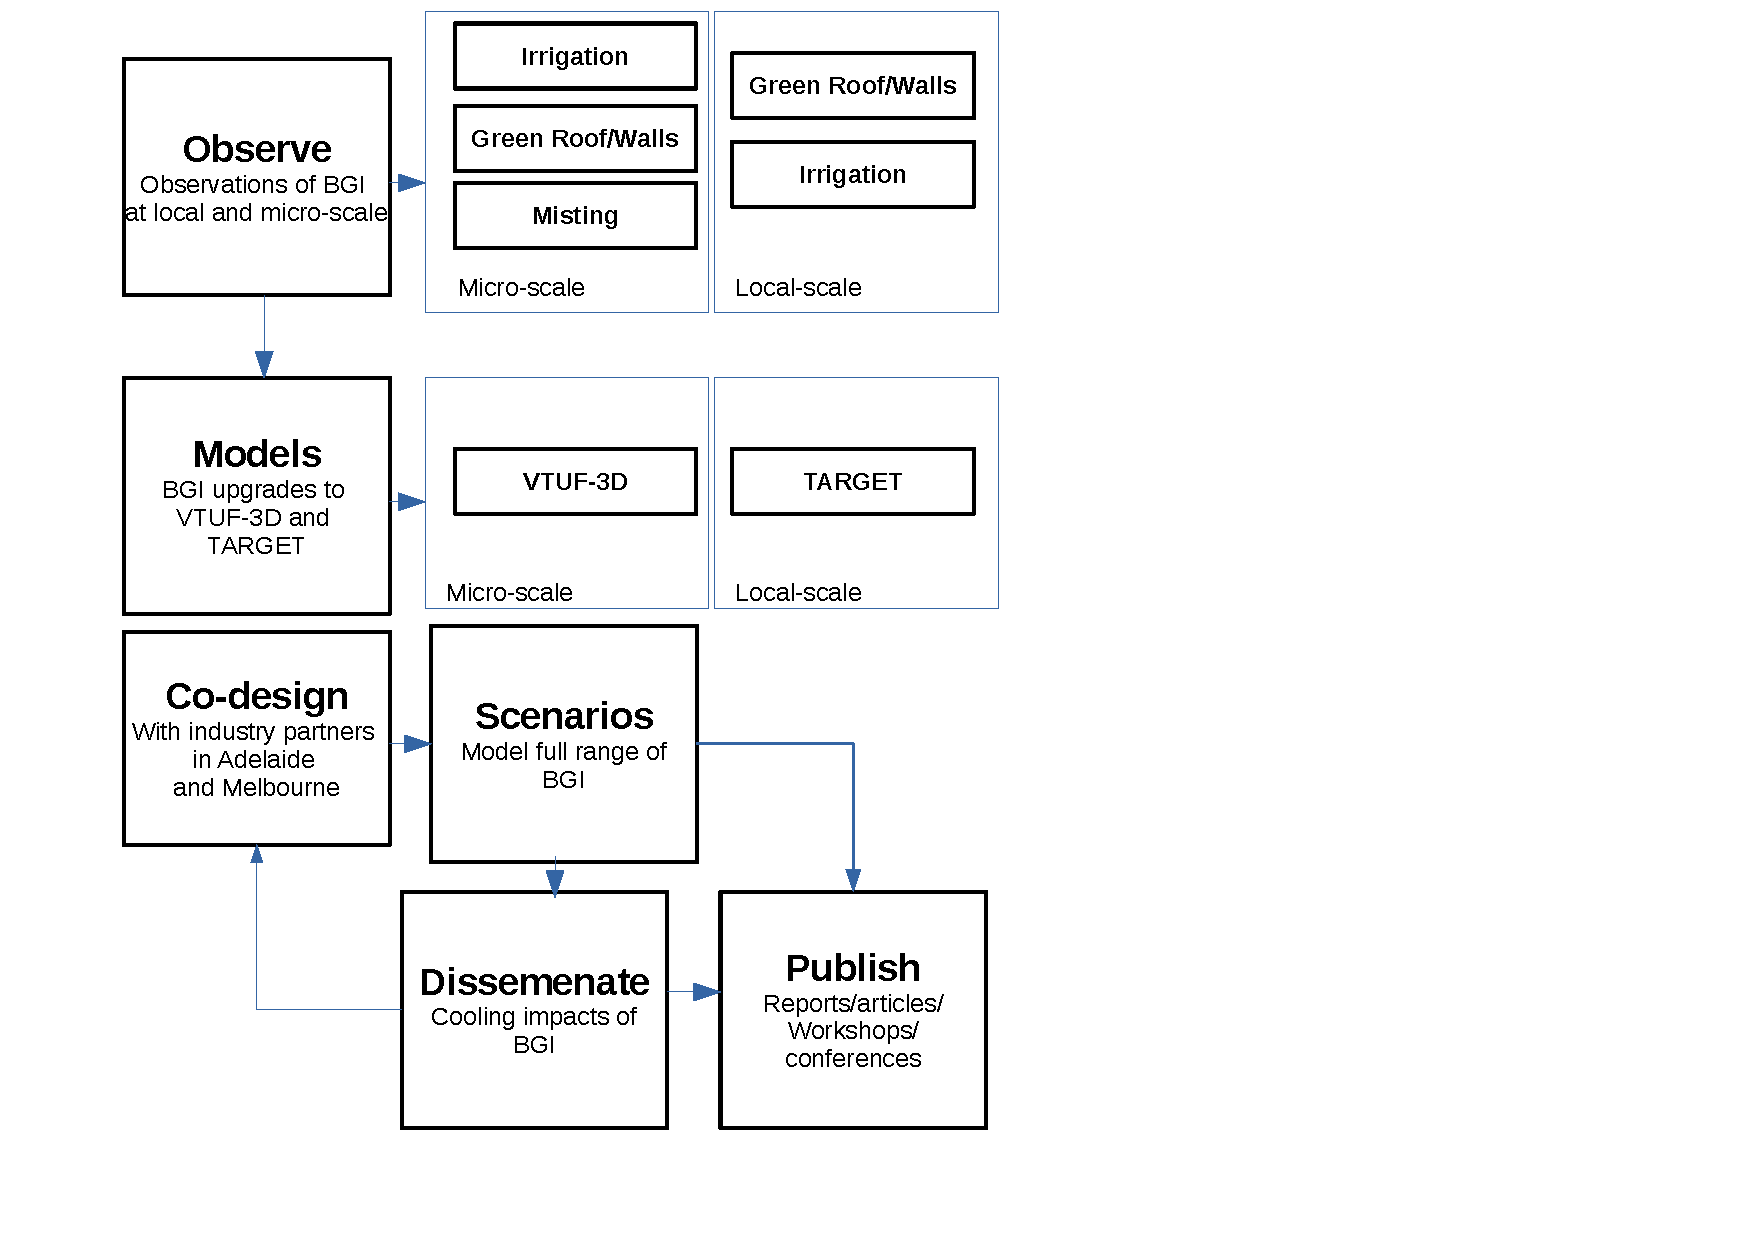
\includegraphics[scale=0.5,trim=40 50 350 0,clip]{Processes.pdf}
}
\end{center}
\caption{Project work packages and steps leading to urban human thermal comfort analysis platform.}
\label{fig:overall}
\end{figure}

\textbf{Work Package 1}: \textbf{Co-design} - \emph{Consult with key stakeholders, especially water companies, to map out the tools and results that will be of highest value to them. }

The first phase of this project will involve a co-design process with industry partners, particularly with South East Water and South Australia Water. I already have an existing working relationship with both. This process will refine the goals and outcomes from the overall research program. Workshops in Adelaide during the first year will be combined with fieldwork travel. Workshops in Melbourne will not require additional travel. Quarterly online meetings will continue throughout the project to ensure this engagement remains on track. In the final year, workshops in Adelaide and Melbourne will be conducted to plan and then integrate the platform and tools into their processes.

\textbf{Work Package 2}: \textbf{Observe} - \emph{Collect observations to supply missing datasets needed to parametrise and validate the modelling of the impacts on human thermal comfort of a wide range of BGI types and water usage practices.}


Two sets of observations have been or are currently being made to enable model development of BGI features. The first set have been collected by Greg Ingleton of South Australia Water. A residential cooling project across Adelaide installed misting system at around 100 residences along with thermometers, flow meters, and soil moisture probes. Surveys have been taken quantifying the effectiveness of the cooling and the impacts on their outdoor behaviour and comfort. A second trial has been conducted within the Adelaide Airport, irrigating a 3.5 hectare site and monitoring the micro-climate over a multi-year period. A second set of observations will be captured in 2020-2021, as part of a project from a PhD student I am currently supervising, across South East Water's Aquarevo housing estate. Micro-climate and detailed soil property observations (air temperature, humidity, incoming and outgoing shortwave and longwave, wind speed and direction, mean radiant temperature and 3 layers of soil moisture and soil temperature) are  to be captured at two sites. The first site is a control site that will be irrigated on a typical suburban schedule. The second site will be irrigated using a number of scenarios, maintaining the soil moisture, emptying rain tanks before rain storms, and irrigating during high heat events. In addition, detailed observations of energy balances, air temperatures and humidity will be observed within a misting system. While both of these datasets are good starting points for some of the following model development and validation, additional data will need to be captured to ensure the full range of BGI can be modelled.

Aquarevo will also be the site of wider precinct scale observations to observe the cooling effects of outdoor water use. Aquarevo is an ideal site for this as they mandate rainwater capture in rainwater tanks that are also remotely controlled to minimise overflows by releasing water before rainstorms or before heatwaves. In addition, each house is fitted with smart water meters, providing detailed usage measurements for drinking, rainwater, and recycled water sources. These observations provide a unique opportunity to understand the cooling benefits of irrigation across both micro- and local-scales and provide data essential to ensure that models are correctly modelling the influence of irrigation across these scales. Further experiments will capture these same observations for patches of turf (5x5m) with daily irrigation (4mm/day) in early morning, or noon, or continuous, or no irrigation (only rainfall). Other patches will test no irrigation, 4mm/day, 8mm/day, and 12/mm day. All the observation instruments for the micro-climate sites have been purchased through South East Water's funding of the current PhD project at Aquarevo. Some additional equipment has been requested in this project's budget to fill in observation gaps in the neighbourhood scaled observations.

\textbf{Work Package 3}: \textbf{Data} - \emph{Process flow for and integration of urban and weather data sources  }

\emph{Urban data:} This work package will assemble a suite of different urban data types, exported from AURIN or WUDAPT, or a process pipeline to convert various types of GIS layers into modelling domain information. These datasets will also be extracted from diverse datasets including Open Street Map, Google Street Map and also from street view and satellite imagery using computer vision and semantic segmentation techniques. Methodology will be devised to combine various sources of urban morphology data from a wide range of providers, including WUDAPT, city inventories, AURIN, and commercial providers into modelling domain input.

For modelling efficiency, a modelling pre-processing step will be devised to define micro-climate zones (MCZ) of representative areas to reduce the amount of areas of a larger modelling domain that need to be individually modelled at a micro-scale. The urban form data can be used as is during the modelling, or can also undergo additional analysis and optimisation. Some parameters necessary for calculating human thermal comfort such as mean radiant temperature can only be properly resolved at a micro-scale, but micro-scaled modelling is computationally expensive. Pre-processing the urban information to find clusters of similar urban typologies can reduce the modelling needed to distinct representative areas for best efficiency.

\emph{Weather data:} The second task is to assemble a suite of forcing weather types, including past BOM observations, ERA5 present observations, BOM ACCESS forecasts, and CIMP5 future climate change projections, and link them into the modelling engine

\textbf{Work Package 4}: \textbf{Models} - \emph{Urban climate modelling tools will be upgraded and shown suitable to model human thermal comfort impacts of BGI and urban water usage.  }

\emph{Improved data interfaces:} The first task is to generate a generic interface to the models to allow a variety of forcing data types (past, present, and future scenarios, including past BOM observations, ERA5 climate reanalysis, BOM ACCESS forecasts, and CIMP5 future climate change projections) to be used and run each within the modelling engine. In the case of TARGET, this will be to adapt the model to be driven with spatial varying weather (compared to having a single weather source driving the entire modelled area). In the case of VTUF-3D, this will be to have instances of VTUF-3D running in parallel in the modelling engine, each with their own weather source. A similar task will be to generate a generic interface to the models to allow the urban design parameters from many different data types to set up the models within the modelling engine.

The other half of the work package will focus on utilising existing observational datasets and acquiring additional observations and using them to upgrade the two models I have previously developed (VTUF-3D and TARGET) and perform validations that they are suitable to model the human thermal comfort impacts of a wide range of BGI features and practices. While VTUF-3D, as a micro-scale model, is more suitable for modelling BGI, upgrades will be performed on both models. The code upgrades will be very similar and most can be applied to both. In addition, as TARGET runs about 100 times faster than VTUF-3D, it can be used first during an analysis process to make first-order estimates to guide subsequent more detailed modelling.  The tasks required are as follows:

To add additional surface types, I propose to utilise two existing models to add these missing components. The first is MAESPA\cite{Duursma2012} which is a soil-plant-atmosphere model that has been previously coupled by myself with the TUF-3D model\cite{Krayenhoff2007} to create the VTUF-3D\cite{Nice2018a} urban micro-climate model. This coupling provides the hydrology and physiological processes of a single tree, a stand of trees, or vegetated irrigated surface cover (i.e. turf) that are currently parameterised in TARGET. To add additional surface types (deep water, swales, misting fountains, porous and/or watered pavements), modules from a second model will be utilised from the Urban Tethys-Chloris (UT\&C)\cite{Meili2020} (co-developed by myself). This model provides a wide range of urban hydrology processes (interception, ponding, vadose zone dynamics, runoff, and soil hydrology) and plant water and biophysical relations. It also allows modelling of many different arrangements of vegetation within the urban canyon including green roofs and green walls. Upgrades will include a simple horizontal advection scheme. These processes are currently neglected for computational reasons. With the addition of this new scheme, wind direction, wind speed, and terrain features will be used to distribute temperature fluxes to nearby grid cells at the end of each timestep. Interfaces need to be created to run both in a modelling engine. This handles processing the urban design information, designing the modelling domain, enabling forcing the different forcing types. Design coupling of the models as online component to regional climate model to allow micro and local-scaled feedback to drive regional changes. An additional change to upgrade VTUF-3D to version 2 is to update the vegetation/hydrology scheme to run online with the model, either through closer coupling with MAESPA\cite{Duursma2012} or total/partial replacement with modules from UT\&C\cite{Meili2020}. 






\textbf{Work Package 5}: \textbf{Platform} \emph{  }

This work package brings together all the work packages into a single ready to use platform. It consists of a number of modules (engines) to complete different parts of the process flow. The first engine is the pre-processing engine to enable integration of micro- and local-climate modelling into city-scale analysis. It brings together the data sources from Work Package 3 and prepares them for submission to the (second) modelling engine. The modelling engine handles the logistics of running the models and storing the results. 

The third engine, the analysis/redesign engine allows analysis on two levels. The first is to provide analysis of the results and methods to compare the results from different scenarios. The second is to enable redesigned scenarios to be iteratively built and recalculated. This will allow setting scenario parameters, design limitations, and ranked priorities to guide redesign efforts. There will be options to manually redesign areas and test the results. These interventions might include increasing the street tree canopy cover, modify irrigation rates, or  conversion of driveways and other hard surfaces to permeable pavement. Redesigned areas are iteratively modelled and analysed to converge on the best designs and discover the significant factors impacting urban heat and generate redesigned areas. Additional analysis will allow adding in layers of urban typologies characteristics and demographics to look at the impacts of the heat modelling results on population health.
 
The final task in this work package is to develop a site that can be used to demonstrate the platform. This will involve packaging the tools and platform into a bundle (such as Docker or Flatpak) so that it can easily be deployed across generic cloud computing servers.







\subsection*{\TitleFont BENEFIT}

%Describe the potential benefits including the:
%- new or advanced knowledge resulting from outcomes of the research;
%- economic, commercial, environmental, social and/or cultural benefits for Australia and
%international communities; and
%- potential contribution to capacity in the Australian Government’s National Science and
%Research Priorities and other priorities identified by government.


The improvements to the models and the analysis platform built around them in this project will deliver benefits on two levels. Their increased sophistication will enable increasingly detailed research to be performed by academic researchers in city science and urban climate. In addition, the platform built around these tools will bring these sophisticated tools to practitioners who need to make immediate decisions about the future design of cities. The tools will also allow assessments to be made about urban heat mitigation and adaptation strategies using vegetation and the use of water practices. The analysis tools can also be used to examine urban areas for hotspots, areas of high vulnerability, that require immediate attention for remediation to reduce the vulnerability and to provide warning to emergency responders and crisis services for areas that might require extra attention during heat waves. This is work that previously could only be performed using expensive and difficult to obtain observations, often incomplete and captured at only a single point in time.

The 2010s was the hottest decade on record and heatwave occurrences and intensities are projected to be even more frequent in the future. The cost of climate change to society will be especially large in urban areas, while the importance of infrastructure planning and management will grow accordingly. This project, with the aim of contributing to better understanding of urban heat and exploring methods to reducing its impact through data acquisition and model development and validation, will help urban planners and city managers to make better, evidence-based decisions, to design better new cities. It will also support the retrofitting of existing areas and design of new more liveable and climate-safe cities. Climate change will also bring new regional weather patterns and understanding how different areas might perform under these new conditions allows better planning future responses to best protect human health.


% how to achieve impact (benefit outside the academy)
% during project
% at end and immediately after
% over next 2-3 years



The benefits will be achieved over a number of stages. The first benefit is the improved urban climate models. That will happen after the first year and those will be enable those benefits to be used by other researchers. This will be integrated into the research of the THUD research lab, as another component in urban design and health. The second stage of benefits results after integrating the tools into the platform following the second year. This will enable working on case studies with industry collaborators. For example, South East Water, Villawood Properties, and Arden Homes have made large investments in designing and building a sustainable and water and energy efficient housing estate and are very interested in being able to showcase the full range of benefits (including cooling using water) to potential customers and to bring sustainable housing into the mainstream. Finally, after the final delivery of the project, the entire platform will be available to a wide range of users. Urban planners, consultants, property developers, among others will be able to test how, where, how much, and what kind of BGI can be used in urban areas to maximise the cooling benefits and create heat resilient cities. As Australian cities become hotter and denser, populations become more elderly and vulnerable to heat risks, these tools will become increasingly important to plan and react to these growing challenges.

\subsection*{\TitleFont FEASIBILITY}

%Describe the:
%- cost-effectiveness of the research and its value for money;
%- feasibility of the research (including contribution of the project’s design, participants
%and resources to the timely completion of the project);
%- supportive environment for the DECRA candidate and their project, and for HDR
%students where appropriate; and
%- availability of the necessary facilities to complete the project.


While developing climate models is complicated and time consuming, my investigator capability demonstrates that I am the ideal person to develop this project. In addition, many of the micro-climate observations needed for the model development and validation will be provided before and during the first stages of this project through an existing PhD supervised project allowing some of the model development to proceed immediately. Additional local-scaled observations can utilise some of the existing equipment through that research project and through support from South East Water to purchase and install. Additional specialised equipment to supplement these has been requested in the equipment budget in this project. All of these datasets will be unique and have many uses outside of their original projects, especially the ones examining the influence of outdoor irrigation on neighbourhood cooling patterns. These observations have not been possible before, without the detailed water usage data that South East Water can provide through the smart meters they have in place across the neighbourhood. Well designed and unique observation datasets can have a long life and be used in a multitude of other research projects. Coutts et al.\cite{Coutts2007} is a perfect example of such a dataset. Adelaide Airport fieldwork will require travel costs to set up, make observations, and disassemble the equipment while Aquarevo work will be performed locally in Melbourne.

Once the modelling tools are created, they can be used for a wide variety of testing scenarios, both analysis of existing places to find vulnerabilities but also testing new ways to design things. This project will design a platform that can be used for demonstration purposes, initially configured for Melbourne and other Australian cities, a `living laboratory', but is also a platform that is transferable to other cities, regions, and countries beyond the end of the project. The funding for these expenses have been requested in the budget for the final year. As I have a high professional and academic interest in the ongoing and continual improvements in the modelling tools I have created, they and the platform they will integrated into will continue past the end of this project. The code for them will always be available through open repositories (i.e. Github or Bitbucket), made available to the international community of urban climate researchers, and the use and development of them will continue through my academic career. Funding has been requested in the budget for urban data costs. Licensing the PSMA Geoscape data will provide the baseline data needed to analyse all the Australian cities in their present form while the Google Street View data will allow the analysis to be expanded to many other locations.

Although the platform will be designed to be user-friendly, some industry engagement, especially with the water companies, through consultation and workshops to work through the documentation process, training, and integration into their design processes in the final year. Travel to Adelaide is included in the budget for this while the rest of the project will be Melbourne based.

At the University of Melbourne, the Transportation, Health and Urban Design Research Lab was created with multi-year seed funding from the university bringing together a large number of researchers from the Faculty around common research themes. This lab provides a very supportive environment for myself and this research. Much of this research can be undertaken in collaboration with other members of this group, and their expertise in research, particularly in the fields of urban analytics, artificial intelligence, and computer vision, is extremely high. Furthermore, the university provides high levels of support to research facilities, including an extensive high performance computing infrastructure (CPU and GPU) with terabytes of available storage. I have gained extensive experience utilising this resource in my research. 

Master's students recruited by the university are generally high quality and many of them have provided valuable research to a number of my past projects. For example, the supervision of three Master's of IT final semester research projects have resulted in methods that were integrated into my 2020 Urban Climate sky pixels publication\cite{Nice2020}. This method of student supervision is an ideal method to provide research experience to Master's students but also to build capacity and gain assistance with development of small discrete portions of this project. However, to mitigate the risk that these projects might produce useful research but that is not directly related to the goals of this project, a modest amount of hours are allocated across the three years for research assistants. In addition, some additional research assistance will be required throughout the project in data analysis and publication preparation.

The overall project plan and timeline are shown in Figure \ref{fig:timeline}

\begin{figure}[ht]
\centering
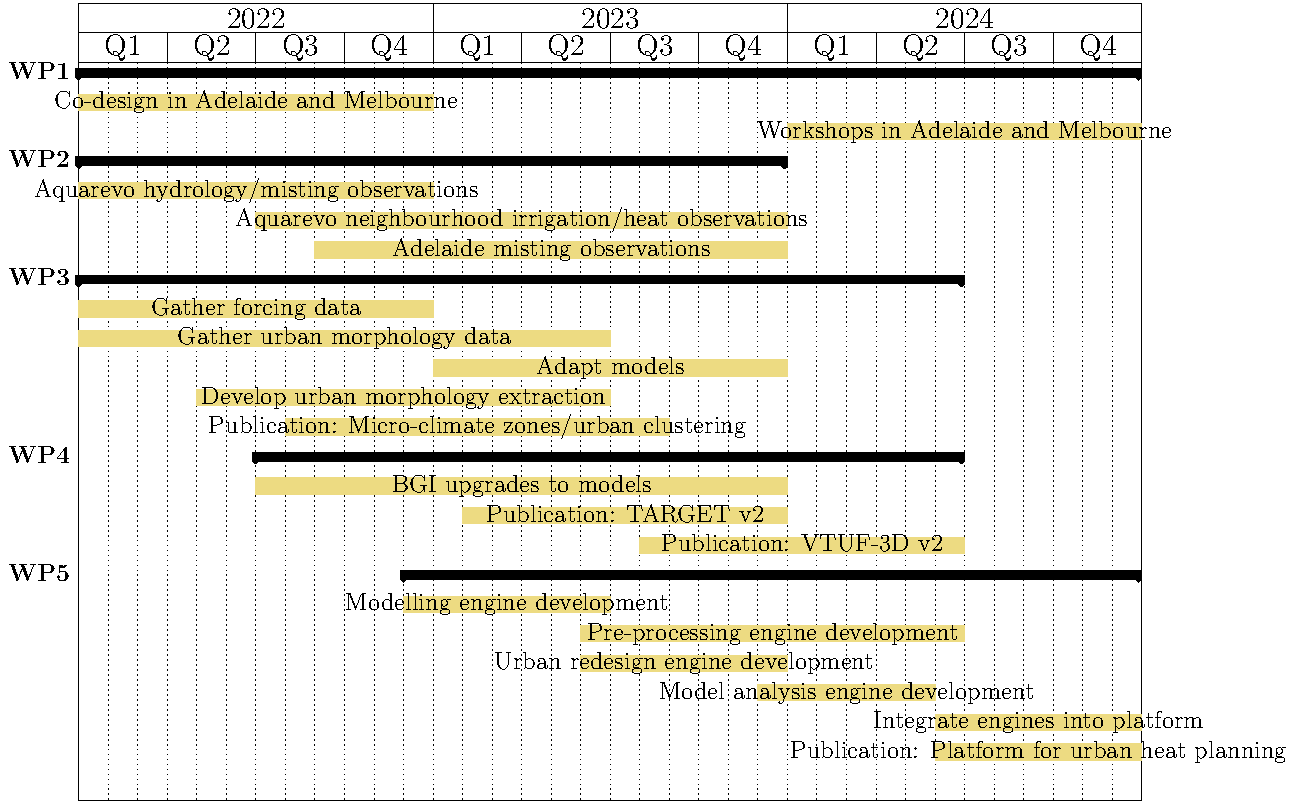
\includegraphics[scale=0.70]{DECRA-D-timeline.pdf}
\caption{Project timeline. }
\label{fig:timeline}
\end{figure}


\subsection*{\TitleFont COMMUNICATION OF RESULTS}

%Outline plans for communicating the research results to other researchers and the broader community, including but not limited to scholarly and public communication and
%dissemination.

There are four peer-reviewed publications planned to result from this project (as well as presented at international conferences including ICUC-11, the AMS General Meeting, and the EGU General Assembly). There will be one article each for the upgrade (v2) of the VTUF-3D and TARGET models, to be likely submitted to the Geoscientific Model Development journal. Another publication will describe the extension of the local climate zone concept into micro-climate zones and how the clustering of those enables and increases the efficiency of doing micro-climate modelling of large areas. It will also describe how to use these distinct types of urban design to identify which types deliver the best thermal performance under extreme heat conditions and what mitigation strategies work best to reduce the risk in vulnerable areas. A further publication will introduce the urban human thermal comfort platform to the urban planning community and perform case studies demonstrating its utility in testing development designs and mitigation strategies. This will involve a stakeholder workshop with previous partners (for example the City of Melbourne or the Victoria Department of Environment, Land, Water and Planning) to test and utilise the platform for some of their current projects. Training documentation and case study results will also be delivered through reports targeted to each of these organisations. 


Beyond academic outputs, translations of the research for more general audiences will be disseminated through platforms such as The Conversation and the University of Melbourne's Pursuit. For example, my recent publication on identifying urban typologies through through the use of urban imagery and computer vision techniques was featured in Pursuit\cite{Nice2020c} and the Sydney Morning Herald\cite{Gladstone2018a}. The platform itself will be demonstrated on an open website as part of this project to allow some testing and experimentation by end users and integrated with industry partners through the project end workshops. The platform will be an open-source bundle will allow other interested users to deploy the platform on their own servers.  




\subsection*{\TitleFont REFERENCES}
\renewcommand{\refname}{\normalfont\selectfont\TitleFont REFERENCES} 
\begingroup
\fontsize{10pt}{10pt}\selectfont
\bibliographystyle{abbrv}


\bibliography{library2}



%Include a list of all references, including relevant references to the previous work of the candidate. References may be in 10 point font.






%\end{document}

\clearpage

 %%! program = pdflatex
%
%\documentclass[12pt,a4paper]{article} 
%\usepackage{arc-dp}
%\usepackage{amsfonts}
%\usepackage{amsmath}
%\usepackage{graphicx}
%\usepackage{times}
%\usepackage{setspace}
%\usepackage{fancyhdr}
%\usepackage{color}
%\usepackage[normalem]{ulem}
%\usepackage{subfig}
%\usepackage{float}
%\usepackage{caption}
%\usepackage{array}
%\usepackage{pgfgantt}
%\usepackage{url}
%\usepackage{enumitem}
%\usepackage{subfig}
%\usepackage{pgfgantt}
%\usepackage{wrapfig}
%\usepackage{enumitem}
%
%\usepackage{booktabs} % for spacing tables
%\usepackage{tabularx} % auto table sizing
%\usepackage{multirow} % table multirow
%\usepackage{soul}
%
%%\usepackage{epsf}
%%\usepackage{fancyheadings}
%%\usepackage{subfigure}
%%\usepackage{pst-gantt}
%%\usepackage{tweaklist}
%
%\newcolumntype{L}[1]{>{\raggedright\let\newline\\\arraybackslash\hspace{0pt}}m{#1}}
%\newcolumntype{C}[1]{>{\centering\let\newline\\\arraybackslash\hspace{0pt}}m{#1}}
%\newcolumntype{R}[1]{>{\raggedleft\let\newline\\\arraybackslash\hspace{0pt}}m{#1}}
%
%\let\OLDthebibliography\thebibliography
%\renewcommand\thebibliography[1]{
%  \OLDthebibliography{#1}
%  \setlength{\parskip}{1pt}
%  \setlength{\itemsep}{1pt plus 0.3ex}
%}
%
%
%%\renewcommand{\enumhook}{\setlength{\topsep}{0pt}%
% % \setlength{\itemsep}{-2mm}}
%%\renewcommand{\itemhook}{\setlength{\topsep}{0pt}%
%%  \setlength{\itemsep}{-2mm}}
%  %%%%%UNCOMMENT THE NEXT COMMAND IF NEEDED
%%\renewcommand{\descripthook}{\setlength{\topsep}{0pt}%
%%  \setlength{\itemsep}{-2mm}}
%
%%\pagestyle{fancy}
%
%%\input{psfig.sty}
%\newcommand{\todo}[1]{\textcolor{red}{#1}}
%\newcommand{\rules}[1]{\textcolor{blue}{#1}}
%\newcommand{\pset}{ {\rm P} \! \! \! {\rm P} }
%\date{}
%%\include{psfig}
%\remove{
%\topmargin -15mm
%\headheight 0pt
%\headsep 0pt
%\textheight 285mm
%\oddsidemargin -15mm
%\evensidemargin -15mm
%\textwidth 190mm
%\columnsep 10mm
%\marginparwidth 0pt
%\marginparsep 0pt
%}
%
%\usepackage[top=0.5cm, bottom=0.5cm, left=0.5cm, right=0.5cm]{geometry}
%\parindent=4mm
%\parskip=0.2mm
%
%%\usepackage{geometry} % see geometry.pdf on how to lay out the page. There's lots.
%%\geometry{a4paper} % or letter or a5paper or ... etc
%% \geometry{landscape} % rotated page geometry
%
%
%%\linespread{1.5}
%
%\newcommand*{\TitleFont}{%
%      \usefont{\encodingdefault}{\rmdefault}{b}{n}%
%      \fontsize{12}{12}%
%      \selectfont}
%
%\title{A unified accessible platform for integration of urban analytics and human thermal comfort modelling}
%%\author{}
%\date{} % delete this line to display the current date
%
%%%% BEGIN DOCUMENT
%\begin{document}
%\rmfamily
%\date{}


\noindent \textbf{F18-ROPE-Details of the participant's academic career and opportunities for research, evidence of research impact and contributions to the field, including those most relevant to this application }\\ \noindent 





\subsection*{\TitleFont Amount of Time as an Active Researcher}

~~~~I was awarded my PhD on urban micro-climate modelling from the School of Earth, Atmosphere and Environment at Monash University in March 2017. I have been an active researcher (at 1.0 FTE) for 4 years and 10 months post-PhD without interruption.

\subsection*{\TitleFont Research Opportunities}

\subsubsection*{\textbf{Academic career}}



~~~~Following a 13 year industry career as a senior and consulting level software engineer (most significantly 8 years at LexisNexis/Reed Elsevier), I returned to university. This previous career has proven highly transferable to my academic research career. It gave me a high level of expertise in software development and design and proficiency in many computer languages (including C++, Python, FORTRAN, and especially Java). I also gained years of experience in project development and management, guiding multi-year projects, developed by globally distributed teams, and delivered to multiple business units around the global. This experience has been directly transferable to managing large research programs, working with remote collaborators, and supervising students.

My post graduate academic career started at the School of Earth, Atmosphere \& Environment  at Monash University. My Master's final semester research project was an observational and modelling study examining the micro-climate of mixed urban and parkland environments which led to engagement by the CRC for Water Sensitive Cities to write a report recommending (but not finding an existing) micro-climate model suitable for thermal comfort impact assessments of water sensitive urban design (especially urban vegetation and water features). My PhD at Monash University followed from this, designing and building this (missing) model. The models VTUF-3D and TARGET resulted from this PhD research and subsequent collaborations with other researchers at Monash. I also designed and built the user interface for the Monash University Simple Climate Model (MSCM) with A/Prof. Dietmar Dommenget (F20, referred articles \#7). This web-based interface (F20, additional research outputs \#17) is a teaching tool that allows students to interactively study the interactions of physical processes in the global climate system through the results of more than a 1000 different model experiments of the Globally Resolved Energy Balance (GREB) model.

My post-doctoral career, at times, has been split (50/50) between two research fellow positions (funded separately) but that encompass research areas that use modelling and computational techniques to examine urban areas for health impacts. One of these position was a 2 year 0.5 FTE research contract (subcontracted through the University of Melbourne) as a Research Fellow and urban climate modelling scientist with Monash University and the CRC for Water Sensitive Cities. My achievements in urban climate model development, even at an early research career stage, have led to recognition as an expert in vegetation and human thermal comfort modelling, leading to this external funding from the CRC for Water Sensitive Cities to further develop this work and consult with local and state government. This role was split between 40\% research, 40\% tool development, and 20\% consulting. 

The research portion was largely devoted to assessments of urban heat outcomes for different urban infill development scenarios. I designed and performed an urban heat analysis of a number of different green field development scenarios in Sunbury for the CRC, especially considering water sensitive (and climate sensitive) urban design. This resulted in a report for the CRC, "Estimating the economic benefits of Urban Heat Island mitigation – Biophysical Aspects" (F20, additional research outputs \#9). Additional modelling analysis of infill development typologies in a number of Australian cities resulted in three additional reports, the `Infill Performance Evaluation Framework', the `Knutsford Urban Heat Modelling Report', and the `Salisbury case study final report: water sensitive outcomes for infill development'. Finally, I wrote the report `Managing urban heat in water sensitive cities: research and policy responses' to summarise the heat mitigation research of the CRC over its eight year program. These reports are additional research outputs \#1-5.

The tool development was devoted to continued development of my urban climate models VTUF-3D and TARGET and their integration with the CRC's scenario planning support tool. I also used this opportunity to improve the performance and usability of my climate models. This is important as very few models can quantify the human thermal benefits of urban green and blue space, especially accounting for cooling effects of vegetation and water evaporation, but often the complexity of configuring, running, and interpreting modelling means this knowledge is out of reach for most potential users.



The consulting included urban heat modelling for state and local government, often joint projects with consulting companies such as GHD. For example, projects resulted in contributions of urban heat assessments to the Urban Ecology Strategy for Fishermans Bend for the Victoria Department of Environment, Land, Water \& Planning (DELWP) and serving on the science panel for the development of the Cool Suburbs Tool for the Western Sydney Regional Organisation of Councils (WSROC). Additional projects include a microclimate assessment for the ACT government and assessments of future heat vulnerability for the Queensland DES/QFES.


\subsubsection*{\textbf{Current roles}}


~~~~My current position is as a Research Fellow (research only)  with the Transport, Heath, and Urban Design (THUD) Research Lab in the Faculty of Architecture, Building, and Planning at the University of Melbourne. This involves research using innovative technologies (artificial intelligence, big data analysis, agent-based modelling, computer vision techniques as well as more traditional statistical methods) to examine multiple aspects of urban areas such as transport networks, urban features, and urban heat and impacts on public health. Building on my PhD research and the position with the CRC, this position incorporates a wide range of disciplines and applies the development and application of modelling to public heath problems. For example, this modelling was applied to a wide range of applications, including modelling of the COVID-19 roadmap for Victoria, creating inventories of cycling infrastructure from remote sensing images, and assessing the impacts of global cities typologies on road injuries. In addition, my software development skills and computer vision technical knowledge has proven highly beneficial to undertaking research across multiple disciplines, leading to new innovations in quantifying health impacts of urban design and transportation infrastructure. This has led to my role as a key contributor to the research lab.

My initial task in THUD was to organise and write an ARC Linkage application, 'A Multi-criteria Design Platform to Facilitate Active School Journeys', quantifying topography, street network connectivity, traffic risk, pollution levels, and thermal comfort. I was not a named participant but the application was submitted in December 2017 (and resubmitted and funded in 2020). I co-developed the neural network clustering and analysis technique used in the lab's recent Lancet Planetary Health publication. This allowed the identification of city types from map segments from the 1700 largest global cities at higher risk of road trauma. This method was expanded in a more recent publication (with myself as first author) in Urban Science to also include street view imagery and satellite imagery to derive urban typologies. Also, in conjunction with other lab collaborators, I developed a method to identify neighbourhood typologies (`block typologies') using self organising maps to cluster metrics extracted from map segments. All three of these projects were used as the base methodology for our lab's current \$1.3 million NHMRC/UKRI research project. My contribution to the lab is also represented in many of the 10 journal publications I co-authored with the lab in the last 4 years.

My expertise in urban heat modelling and computer vision techniques have led to me being sought out to participate as a co-investigator a \$422,000 ARC Discovery (fully detailed below) to create cycling risk exposure models from satellite and street view imagery and from Strava data and traffic cameras. I am also a co-investigator on an awarded 453,764 CHF Swiss National Science Foundation grant `Heat-Down: Integrated modelling of stormwater and urban heat for cooling cities' headed by Dr. Jo\~{a}o P. Leit\~{a}o (Eawag) and Dr. Peter M. Bach (ETH Zurich) based on my TARGET model. I have also built on an ongoing collaboration with the UNSW City Futures Research Centre with a recently submitted application for the AURIN High Impact Projects 2021, `Climate Resilient and Just Cities: Data for Research and Practice' led by Dr. Negin Nazarian.

At the University of Melbourne, Prof. Mark Stevenson (professor of Urban Transport and Public Health and NHMRC Research Fellow) supervises my other position and along with other members of the lab (especially Dr. Jason Thompson, the senior research fellow in the lab) provides valuable mentoring. Through my academic career, I have been fortunate to receive excellent mentoring and career guidance. My PhD was supervised by Prof. Nigel Tapper (Monash University; current president of The International Association for Urban Climate) and Dr. Andrew Coutts (Monash University; a leading urban climate researcher). Prof. Tapper remains a frequent collaborator and co-supervisor of honours and PhD students. 




\subsection*{\TitleFont Research Achievements and Contributions}

\textbf{How my research has led to advances in knowledge in the field. How will my achievements contribute to the application:}


As an early-career researcher, I have quickly built a large body of work. These research achievements include a number of urban climate models able to examine urban heat mitigation strategies at local and micro-scales and make predictions of human thermal stress. These models have been adopted by other researchers and consultants. My knowledge about modelling and model development has led to being included in research projects and grant applications to further develop these models and contribute to the development of other models. In addition, methods that I have developed using computer vision techniques to cluster similar types of urban areas and examine the links of the design to public health outcomes and have formed the basis of successful grant applications and research papers. These techniques and the results from them (especially those around urban heat) are currently being utilised by state and local governments to formulate appropriate public health measures.

After my industry career and PhD candidacy, I have focused on building and improving my track record as a researcher. Despite having completed my PhD by thesis and as a result my research has only started to be published in 2018, when comparing with other researchers in urban climate modelling and model development at similar stages of their careers, my publication output compares favourably (Figure \ref{fig:benchmark}). When comparing citation counts, my record shows a rapidly rising trajectory in the last four years (in Google Scholar, 13 in 2019, 60 in 2020, and 90 in 2021), but it should also be considered that citations take a number of years to accumulate.



\begin{wrapfigure}{r}{0.65\textwidth}
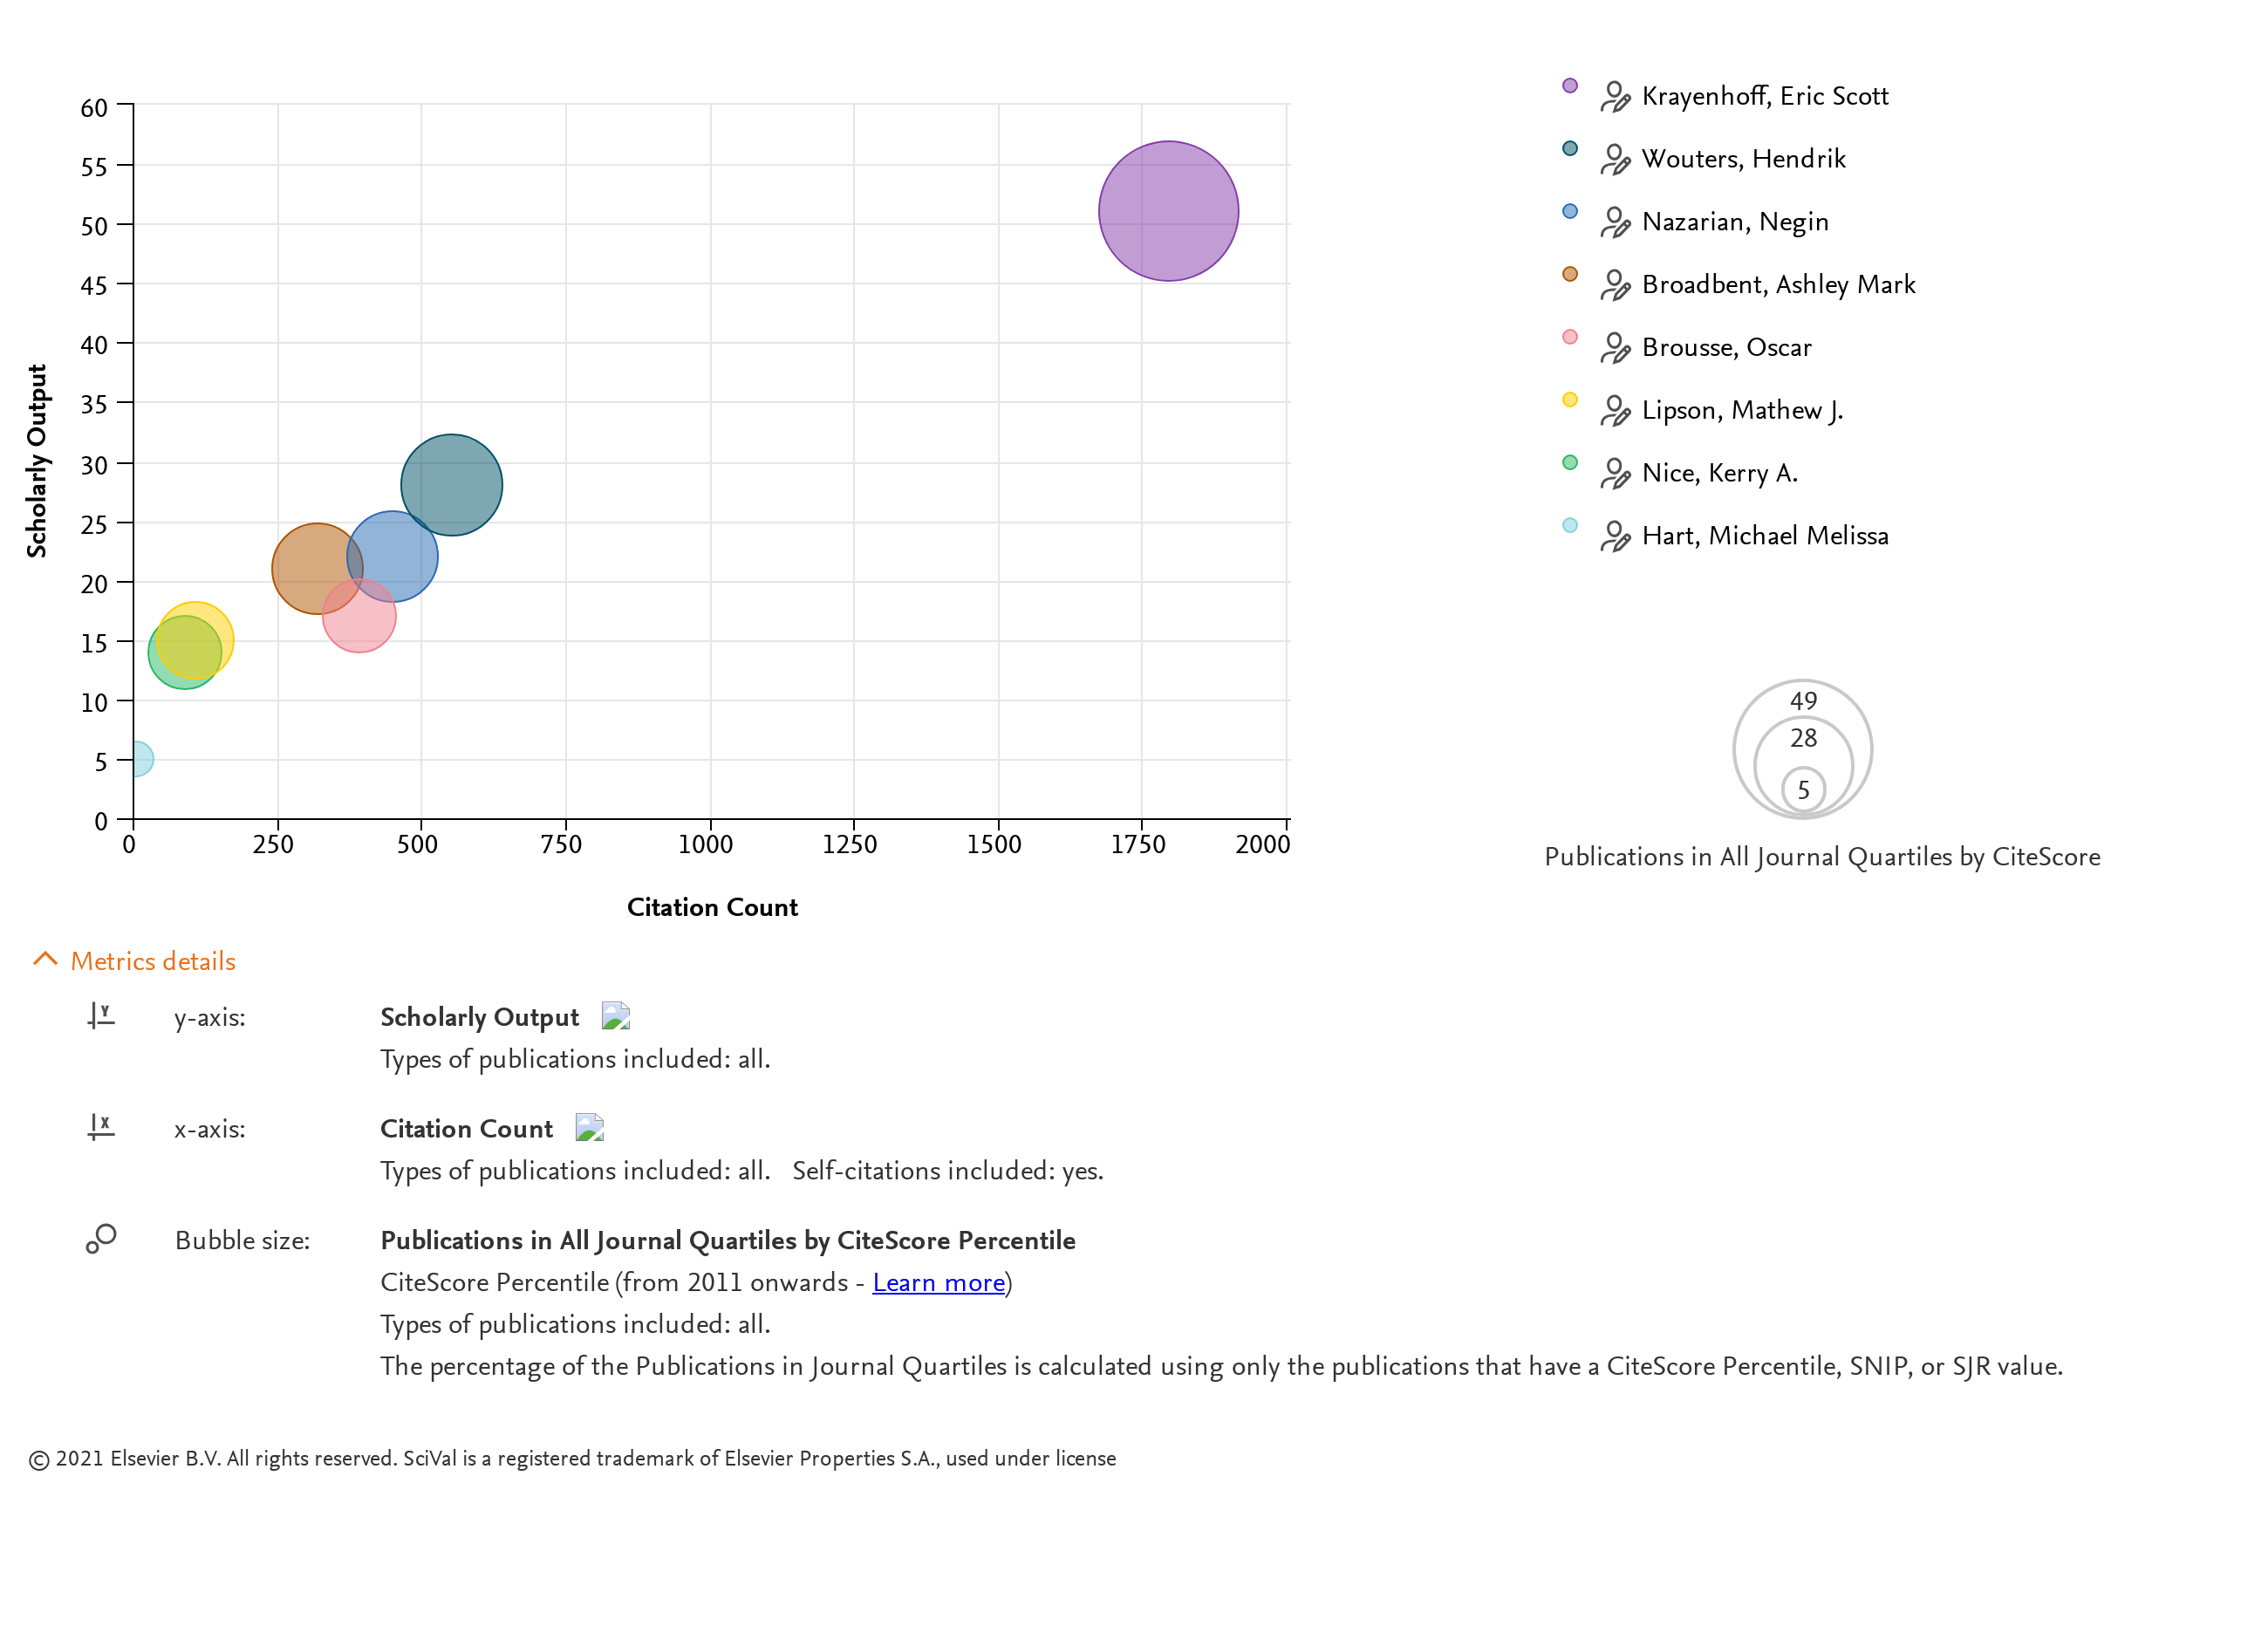
\includegraphics[trim={20 800 150 20},clip,scale=0.12]{metrics/K-Nice-2-2021.png}
\caption{Benchmarking of my publication output in top 10\% journals (by CiteScore percentile) compared to well-regarded researchers in urban climate modelling and model development at similar stages of their careers. Y-axis: All types of publications included. Bubble size: CiteScore percentile (from 2011 onward) (Source: Elsevier SciVal).}
\label{fig:benchmark}
\end{wrapfigure}


The first stage of my academic career has been in urban climate modelling, the topic of my PhD. The model I developed in my PhD, VTUF-3D remains one of the few models able to assess the cooling impacts of urban vegetation at a micro-scale, and has led to further collaborations and model development as well as a large engagement. My PhD thesis, from which the journal article was developed, has had over 2,000 reads. Three additional climate models, TARGET, UT\&C, and MSCM-DB, have been co-developed through collaborations. In a collaboration (F20, top 10 \#8), have explored the state of the art in modelling (including my VTUF-3D model) outdoor mean radiant temperatures, a key parameter for predicting heat stress, and found circumstances where VTUF-3D and ENVI-met successfully model this parameter and where they encounter challenges. 

My recent paper in Sustainable Cities and Society, `Estimating the cooling potential of irrigating green spaces' is directly related to this DECRA application. In addition, my research in urban heat has also included wider multidisciplinary applications of (and a framework around) water usage and urban design on both urban heat and other issues of urban liveability that were presented at the State of Australian Cities conference (\#2 below). I have utilised computer vision techniques in support of urban climate modelling. This led to a method to more accurately detect sky pixels (a preliminary step in calculating sky view factors) using a range of urban imagery types (F20, top 10 \#4). I presented methods to utilise urban morphology databases (such as WUDAPT) in conjunction with micro-climate modelling to target heat mitigation strategies and the beginning steps to discover and define micro-climate zones at the European Geosciences Union conference EGU2020 (\#3 below). This has been expanded to an (in-progress) collaboration with researchers at UNSW to isolate the impacts of urban form and fabric from geography on heat mitigation strategies.

While my expertise in urban climate and urban climate modelling have the most direct link to the successful delivery of this project, much of my recent research has involved the use of artificial intelligence and machine learning. These techniques can be applied to urban climate questions as well. The \$30,000 2020 Melbourne Energy Institute grant resulted in a study (currently in review with Atmospheric Pollution Research) using XGBoost to quantify the effects of human activity (reduced during COVID-19) on key pollutants (NO$_{2}$, PM$_{2.5}$, PM$_{10}$, and O$_{3}$) across 700 global cities. Other research has included using neural networks to cluster the largest 1700 global cities using millions of maps and examine the impact of urban design types on road trauma, as well as adding additional imagery types (satellite and street view) to the maps to construct urban typologies based on features discovered in the imagery. I've used other types of artificial intelligence, generative adversarial networks, to transform street level and satellite imagery from areas with poor health outcomes into new imagery, providing insights into the urban factors leading to these poor outcomes. Finally, I have used deep autoencoder extracted features from satellite imagery of all the intersections in Australia to identify safe intersection design. 

In addition, my record of publication in high impact journals have also given me an understanding of complex review processes and required engagement in international-level debates. The Computer-Aided Civil and Infrastructure Engineering publication required satisfying 10 reviewers. The Lancet Planetary Health publication, with a multi-year review process and an excess of 10 reviewers, proved even more challenging. Numerous editorials are published in public health about the need to develop and utilise new techniques and multi-disciplinary approaches, but actually submitting this work requires overcoming large amounts of resistance to moving beyond what has always been done.

I have presented my research at 8 international conferences and 7 national conferences with 3 of those as invited talks. My research has also been featured in 5 collaborative presentations at 5 international conferences (1 as an invited talk). 

The following conference presentations and conference papers are most strongly related to this DECRA application (i.e. climate model development, human thermal comfort modelling, and the collection of urban morphology information through databases and extraction from urban imagery).

\begin{list}{}{}
\itemsep-0.5em

\item [1.] G\'{a}l, C. V and \textbf{Nice, K. A.} ‘Mean radiant temperature modeling outdoors: A comparison of three approaches’, in \textit{100th Annual Meeting of the American Meteorological Society (AMS) jointly with the 15th Symposium on the Urban Environment}, 2020. 
\item [2.] Todorovic, Tatjana, London, Geoffrey, Bertram, Nigel, Sainsbury, Oscar, Renouf, Marguerite A, \textbf{Nice, Kerry A} and Kenway, Steven J. 2019. ‘Models for water sensitive middle suburban infill development’, in\textit{ 9th State of Australian Cities National Conference, 30 November - 5 December 2019, Perth, Western Australia}. doi: 10.25916/5efa774bda643. 
\item [3.] \textbf{Nice, K. A.}, Targeted urban heat mitigation strategies using urban morphology databases and micro-climate modelling to examine the urban heat profile. \textit{EGU General Assembly 2020}.

\end{list}

Further other research outputs support my expertise in urban climates, urban typology clustering and urban analytics.
\begin{list}{}{}
\itemsep-0.5em
\item [4.] \textbf{Nice, K. A.}, Climate science context around urban cooling. In: \textit{4th Water Sensitive Cities Conference 2019, Brisbane}. \textbf{Invited talk.}
\item [5.] \textbf{Nice, K. A.}, Urban Greening for improved human thermal comfort. In: \textit{202020 Vision, The Green Light Tour, 2018, Adelaide}. \textbf{Invited talk.}
\item [6.] \textbf{Nice, K. A.}, Designing liveable cities through heat mitigation: tools to translate knowledge into design. In: \textit{3rd Water Sensitive Cities Conference, 2017, Perth.} \textbf{Invited talk.}
\item [7.] \textbf{Nice, K.A.}, The Nature of Human Settlement: Building an understanding of high performance city design. In: \textit{UrbanSys2019/2019 Conference on Complex Systems, Singapore.}
\end{list}

I have developed a strong collaborative network (within my universities, Australia, and internationally), and developed a strong research direction based on modelling and quantifying urban systems. This rapid upward trajectory has been strongly enabled by a previous long career in industry and software engineering that required the ability to develop and organise large projects, solve problems, and build the tools necessary to deliver results. This combination of extensive experience in computing techniques with deep urban climate and urban climate modelling development knowledge demonstrate that I am the ideal researcher to undertake and deliver this project.


\textbf{Invited keynote and speaker addresses:}

I have presented my research at 8 international and 7 (3 invited, \#4, \#5, and \#6 above) national conferences since 2012. Three of these have been at the International Conference on Urban Climate (ICUC), the leading conference for urban climate. Two of these ICUC talks were about my VTUF-3D model and one was about using computer vision techniques and Google Street View to discover urban morphology parameters (namely sky view factors). Two recent international conference presentations have been on the topic of deriving urban typologies through big data urban imagery datasets and machine learning and computer vision. I have given three invited presentations on the topics of urban heat and designing heat mitigation strategies at the 3rd and 4th Water Sensitive Cities Conferences in Perth and Brisbane and in the 202020 Vision Green Light Tour in Adelaide (202020 Vision is now Greener Spaces Better Places). I have also been invited to present five guest lectures at Monash University and the University of Melbourne on the topic of urban climate modelling and the urban heat benefits of water sensitive urban design. 

\textbf{Research income:}

I have secured AUD \$1,207,910, GBP \textsterling479,387, and 453,764 CHF in research income through competitive grants over the last five years. This demonstrates my capacity to secure funding across a wide range of research areas in collaboration with other Australian and international researchers and delivering publications and reports from these projects.

\begin{itemize}
\item In 2016 I was awarded the \$10,000 Graham Treloar Early Career Researcher Fellowship (The University of Melbourne Faculty of Architecture, Building and Planning) for the development of the project `Urban canyon mean radiant temperatures predictions through mining Google Street View imagery and neural network machine learning'. The outcome from this project was published in career-best publication \#4.

\item I am a Co-Investigator on the AUD \$608,910 (and GBP \textsterling479,387) 2020-2023 UKRI/NHMRC grant 1194959, `A Vision of Healthy Urban Design for NCD Prevention'. The methodology for this grant utilises neural networks and computer vision techniques to process large amounts of urban imagery to assess the impacts of urban design on non-communicable disease (NCD). This is a collaborative project between researchers at the University of Melbourne and Queen's University Belfast.

\item I secured a \$137,000 research contract with the CRC for Water Sensitive Cities as a specialist cohort in urban heat modelling. This contract was solicited by the CRC to provide urban heat expertise to the final two years of the CRC research program and provides two years of 0.5 FTE funding over 2019-2020. This funding has provided opportunities both to advance my model development work and work in collaboration with industry partners and local and state governments to develop urban heat mitigation strategies (as detailed in the benefits section below).

\item I am a Chief Investigator on a \$30,000 2020 Melbourne Energy Institute grant on `The effects of COVID-19 on reduced transport and emissions for global city typologies'. 

\item I am a Chief Investigator on the \$402,000 2021-2023 ARC Discovery DP210102089 `Sustainable mobility: city-wide exposure modelling to advance bicycling' grant headed by Dr Ben Beck (Monash University). This grant utilises my expertise in computer vision and machine learning to extract an inventory of cycling infrastructure from satellite and street view imagery. These inventories will be used to develop a platform for city-wide modelling of cycling exposure that can be applied globally.

\item I am a Partner Investigator on a 453,764 CHF 2021 Swiss National Science Foundation Project ID 200021\_201029, `Heat-Down: Integrated modelling of stormwater and urban heat for cooling cities'. My urban climate model, TARGET, will be upgraded and utilised to investigate heat mitigation strategies enabled by the use of stormwater.

\end{itemize}




\textbf{Research supervision, mentoring and advice:}


Student supervision of topics closely related to this project has provided experience in micro-climate observations of cooling through BGI features. I am currently co-supervising two PhD students in conjunction with Prof. Nigel Tapper (Monash) and A/Prof. Stephen Livesley (Melbourne). The student at Monash University/Southeast University is observing and modelling the cooling potential of irrigation of the runway buffer areas at Adelaide Airport. Another student at the University of Melbourne is looking at the cooling potential and energy balances of misting systems and irrigation of turf grass and trees. I am supervising one Honours student at Monash in conjunction with Prof. Nigel Tapper and Prof. Julie Arblaster, who will be modifying VTUF-3D to include the ability to model impervious surfaces watering based on an observation campaign.

I have also supervised the final capstone research projects for 11 Masters of IT (MIT) students at the University of Melbourne. Methods from 3 of these MIT projects were incorporated into the Urban Climate paper, listed above. In addition, methods from one other MIT project is currently being incorporated into a health/computer vision collaboration with researchers from Cambridge University. Finally, I have been invited to participate in 3 PhD review panels for the urban climate discipline.



\textbf{Benefits outside academia:}

My expertise in urban heat modelling has been utilised in a number of government consultations and planning reports in 2019-2021. I am currently consulting with the Department of Agriculture, Water and the Environment (DAWES) for the project 'Health cost impacts of urban heat amelioration through integrated water cycle management (IWCM) measures', a consortium through Marsden Jacob with a modelling team led by Prof. Nigel Tapper (Monash) with Dr. Andrew Coutts, and Dr. Matthias Demuzere (RUB) and a health team led by Prof. Peng Bi (University of Adelaide). Past projects include serving on the science advisory panel for Western Sydney Regional Organisation of Councils (WSROC) Cool Suburbs Rating and Accreditation tool, providing modelling and urban heat analysis for the Queensland Department of Environment and Science (DES), reports for urban heat impacts of infill development for South Australia (Salisbury, an Adelaide suburb) and Western Australia (the Perth suburb of Kutsford), urban heat assessments for the Fishermans Bend Urban Ecology Strategy for the Victorian government, and project work for the ACT government's micro-climate urban heat strategies.



\textbf{Other professional activities:}

I maintain memberships in the European Geosciences Union (EGU), The Australian Meteorological and Oceanographic Society (AMOS), The International Association for Urban Climate (ICUC), and the Complex Systems Society (CSS).

Article Referee Activities: In the past 5 years, I have performed 45 peer reviews for 17 leading climate and urban design journals, including Urban Climate, Theoretical and Applied Climatology, Sustainable Cities and Society, Environmental Science \& Technology, Environment and Planning B, Scientific Reports, Science of the Total Environment, Landscape and Urban Planning and am on the review board for Atmosphere.




%\end{document}

\clearpage

%


%! program = pdflatex
%
%\documentclass[12pt,a4paper]{article} 
%\usepackage{arc-dp}
%\usepackage{amsfonts}
%\usepackage{amsmath}
%\usepackage{graphicx}
%\usepackage{times}
%\usepackage{setspace}
%\usepackage{fancyhdr}
%\usepackage{color}
%\usepackage[normalem]{ulem}
%\usepackage{subfig}
%\usepackage{float}
%\usepackage{caption}
%\usepackage{array}
%\usepackage{pgfgantt}
%\usepackage{url}
%\usepackage{enumitem}
%\usepackage{subfig}
%\usepackage{pgfgantt}
%\usepackage{wrapfig}
%\usepackage{enumitem}
%
%\usepackage{booktabs} % for spacing tables
%\usepackage{tabularx} % auto table sizing
%\usepackage{multirow} % table multirow
%\usepackage{soul}
%
%%\usepackage{epsf}
%%\usepackage{fancyheadings}
%%\usepackage{subfigure}
%%\usepackage{pst-gantt}
%%\usepackage{tweaklist}
%
%\newcolumntype{L}[1]{>{\raggedright\let\newline\\\arraybackslash\hspace{0pt}}m{#1}}
%\newcolumntype{C}[1]{>{\centering\let\newline\\\arraybackslash\hspace{0pt}}m{#1}}
%\newcolumntype{R}[1]{>{\raggedleft\let\newline\\\arraybackslash\hspace{0pt}}m{#1}}
%
%\let\OLDthebibliography\thebibliography
%\renewcommand\thebibliography[1]{
%  \OLDthebibliography{#1}
%  \setlength{\parskip}{1pt}
%  \setlength{\itemsep}{1pt plus 0.3ex}
%}
%
%
%%\renewcommand{\enumhook}{\setlength{\topsep}{0pt}%
% % \setlength{\itemsep}{-2mm}}
%%\renewcommand{\itemhook}{\setlength{\topsep}{0pt}%
%%  \setlength{\itemsep}{-2mm}}
%  %%%%%UNCOMMENT THE NEXT COMMAND IF NEEDED
%%\renewcommand{\descripthook}{\setlength{\topsep}{0pt}%
%%  \setlength{\itemsep}{-2mm}}
%
%%\pagestyle{fancy}
%
%%\input{psfig.sty}
%\newcommand{\todo}[1]{\textcolor{red}{#1}}
%\newcommand{\rules}[1]{\textcolor{blue}{#1}}
%\newcommand{\pset}{ {\rm P} \! \! \! {\rm P} }
%\date{}
%%\include{psfig}
%\remove{
%\topmargin -15mm
%\headheight 0pt
%\headsep 0pt
%\textheight 285mm
%\oddsidemargin -15mm
%\evensidemargin -15mm
%\textwidth 190mm
%\columnsep 10mm
%\marginparwidth 0pt
%\marginparsep 0pt
%}
%
%\usepackage[top=0.5cm, bottom=0.5cm, left=0.5cm, right=0.5cm]{geometry}
%\parindent=4mm
%\parskip=0.2mm
%
%%\usepackage{geometry} % see geometry.pdf on how to lay out the page. There's lots.
%%\geometry{a4paper} % or letter or a5paper or ... etc
%% \geometry{landscape} % rotated page geometry
%
%
%%\linespread{1.5}
%
%\newcommand*{\TitleFont}{%
%      \usefont{\encodingdefault}{\rmdefault}{b}{n}%
%      \fontsize{12}{12}%
%      \selectfont}
%
%\title{A unified accessible platform for integration of urban analytics and human thermal comfort modelling}
%%\author{}
%\date{} % delete this line to display the current date
%
%%%% BEGIN DOCUMENT
%\begin{document}
%\rmfamily
%\date{}

\subsection*{\TitleFont F19. Research Opportunity and Performance Evidence (ROPE) - Research Output Context - Research context: }

\textbf{Provide clear information that explains the relative importance of different research outputs and expectations in the participant's discipline/s. The information should help assessors understand the context of the participant's academic research achievements but not repeat information already provided in this application. It is helpful to include the importance/esteem of specific journals in their field; specific indicators of recognition within their field such as first authorship / citations, or significance of non-traditional research outputs. (Up to 3,750 characters, approximately 500 words).)}

I currently have published 14 journal articles (3 as first author and 3 as second author) and 3 refereed full-length conference papers. In the four years that I have been publishing (since 2018), I have already accumulated 181 citations in Google Scholar and a h-index of 7. My citations are increasing rapidly, with 90 of them occurring in 2021. The article on my VTUF-3D model is my most cited work. I have 7 reports written for the CRC for Water Sensitive Cities and 1 book chapter. My publication output compares favourably (as shown in F18) to a selection of other highly respected urban climate researchers at similar or later career stages. 

My research crosses a number of different disciplines, urban climates, climate modelling, artificial intelligence, computer vision, urban analytics, urban design, and public health. For all the fields I have published in, authorship conventions are similar, ordered by contribution level, with the first author leading the effort, the second and third authors generally also making large contributions, and the final author supervising. Sole authorship is rare because of the collaborations and inter-disciplinary research required in these areas.

There are a wide variety of climate journals but Urban Climate (SJR Q1 1.151) is the central journal for urban climate. Geoscientific Model Development (SJR Q1 3.238) is a leading journal modelling and simulation, especially geophysical modelling development. Author lists can include 5-10 authors as model development is an incremental process and next generation models generally build on the work of previous models.

The computer vision and artificial intelligence fields publish predominately in conference proceedings, but applied research is more often published in domain specific journals. My other research outside of urban climates generally crosses multiple disciplines and is published in interdisciplinary orientated journals. Lancet Planetary Health (SJR Q1 4.205) is a highly ranked interdisciplinary journal covering global health issues. Sustainable Cities and Society (SJR Q1 1.65) focuses on multi-disciplinary research into designing resilient cities. Q1 journal Environment and Planning B focuses on state of the art analytical methods for urban planning and design. Computer-Aided Civil and Infrastructure Engineering (Q1 SJR 2.77) focuses on the the use of computer science in aid of engineering.

Many papers have attracted attention. Five received an Altmetric Attention Score of 10 or higher. Seven are over 5. The Lancet Planetary Health paper has a score of 165, the streetscape augmentation paper has reached 20, and the Urban Science paper 17.

Conferences in my various disciplines are either a combination of abstract submission and presentation or abstract submission, presentation, and then a fully peer-reviewed article in the proceedings. I have participated in both types. A peer-reviewed article resulted from three, the American Meteorological Society, the State of Australian Cities, and Digital Image Computing conferences.

Other research outputs from my career are made up of modelling code (the four models I have developed or co-developed) distributed through online public repositories. DOI numbers can be assigned to attract citations when the code is used by others, but in practice the code is rarely given recognition on its own and are only cited in other's academic work via the publications describing their development. Usage or adoption by consultants or other non-academic users will generally receive no public recognition.















%\end{document}

\clearpage




\end{document}

